% options:
% thesis=B bachelor's thesis
% thesis=M master's thesis
% czech thesis in Czech language
% slovak thesis in Slovak language
% english thesis in English language
% hidelinks remove colour boxes around hyperlinks

\documentclass[thesis=B,czech]{FITthesis}[2017/05/04]

\usepackage[utf8]{inputenc} % LaTeX source encoded as UTF-8

\usepackage{graphicx} %graphics files inclusion
% \usepackage{amsmath} %advanced maths
% \usepackage{amssymb} %additional math symbols

\usepackage{dirtree} %directory tree visualisation
\usepackage{listings}
\usepackage{minted}
\usepackage{rotating}

% % list of acronyms
% \usepackage[acronym,nonumberlist,toc,numberedsection=autolabel]{glossaries}
% \iflanguage{czech}{\renewcommand*{\acronymname}{Seznam pou{\v z}it{\' y}ch zkratek}}{}
% \makeglossaries

\newcommand{\tg}{\mathop{\mathrm{tg}}} %cesky tangens
\newcommand{\cotg}{\mathop{\mathrm{cotg}}} %cesky cotangens

% % % % % % % % % % % % % % % % % % % % % % % % % % % % % %
% ODTUD DAL VSE ZMENTE
% % % % % % % % % % % % % % % % % % % % % % % % % % % % % %


\department{Katedra počítačových systémů}
\title{Infrastruktura pro centralizovanou automatickou instalaci serverů}
\authorGN{Jan} %(křestní) jméno (jména) autora
\authorFN{Sokol} %příjmení autora
\authorWithDegrees{Jan Sokol} %jméno autora včetně současných akademických titulů
\supervisor{Ing. Jiří Dostál}
\acknowledgements{Rád bych poděkoval mému vedoucímu práce Ing. Jiřímu Dostálovi za jeho opakovanou pomoc jak se strukturou bakalářské práce, tak i obsahem. Osoby v~následujícím výčtu mi velmi pomohly v~nejhorších chvílích, kdy se psaní zdálo skoro nemožné. Jmenovitě maminka Monika Sokolová, sestra Markéta Sokolová a Milica Marić. V~neposlední řadě Anuša Kovačič, Henrich Le, Davor Miletić, Denys Sidorenko, Jakub Tobolka, Vanja Djurdjevic, Tomáš Hyhlík a další, kteří se mnou bakalářskou práci konzultovali.}

\abstractCS{Tato bakalářská práce se zabývá průzkumem a implementací systému na~instalaci serverů bez~lidského dozoru. Cílem práce je využití některého již použitého systému a s~úpravami nasazení do produkce. V~teoterické části práce je popsána analýza 5 vybraných nástrojů. Mezi kritéria výběru těchto nástrojů patřilo z~ekonomických a praktických důvodů open-source řešení, dále rozvinutá komunita, jež může pomoci s~řešením případných problémů s~nástrojem. Na základě analýzy z~předchozí části  byl vybrán nástroj, který nejlépe vyhovoval stanoveným požadavkům: jednoduše použitelné grafické rozhraní, podpora instalace široké škály operačních systémů (podmínkou alespoň OS Debian a CentOS) a možnost rychlých úprav v~konfiguracích instalovaných serverů. Následovně je popsáno nasazení vyhovujícího nástroje Foreman, jak hlavního uzlu, tak proxy serverů v~oddělených lokalitách. V~další části je popsán vývoj a nasazení pluginu v~prostředí Foreman, který v~jeho grafickém rozhraní zobrazuje grafy z~dat sesbírané démonem collectd. Práce také obsahuje konfigurační skripty pro Ansible pro jednoduché zprovoznění serverů.}

\abstractEN{This thesis deals with research and deployment of provisioning frameworks for bare metal servers. Goal of this thesis is to chose one of those frameworks, deploy it and with changes use it in production. The choosing criteria are: open-source software for practical and economical reasons, comunity behind framework and support for installed operating system (there has to be at least OS CentOS and Debian). Based on analysis in the first chapter was chosen framework Foreman, that suits criteria the best -- simple and usable graphical web interface, support for multiple separated local area networks and an option to change configuration of installed systems fast. Another chapter shows deployment of Foreman framework. This thesis also includes plugin for Foreman to show graphs from rrd data source (with use of Collectd Graph Panel). Ansible playbooks for simple deployment of Foreman servers are also included. }


\placeForDeclarationOfAuthenticity{V~Praze}
\declarationOfAuthenticityOption{4} %volba Prohlášení (číslo 1-6)
\keywordsCS{linux, foreman, provisioning, server, bare metal, plugin, ansible}
\keywordsEN{linux, foreman, provisioning, server, bare metal, plugin, ansible}

\begin{document}

% \newacronym{CVUT}{{\v C}VUT}{{\v C}esk{\' e} vysok{\' e} u{\v c}en{\' i} technick{\' e} v Praze}
% \newacronym{FIT}{FIT}{Fakulta informa{\v c}n{\' i}ch technologi{\' i}}


\begin{introduction}
Jakýkoliv hardware spojovaný s~počítači, dříve než začne vykonávat svoji činnost, vyžaduje mít nainstalovaný a správně nakonfigurovaný software. Příkladem může být obyčejný stolní počítač, který potřebuje v~sobě mít nainstalovaný operační systém spolu s~ovladači. Tato instalace spolu s~následující konfigurací může být časově poměrně náročná. Pokud ale těchto počítačů, potažmo serverů bez nainstalovaného operačního systému (pozn. v~angličtině bare metal machine) máme desítky, dokonce stovky, čas vložený do instalace těchto strojů se může vyšplhat na neúnosné číslo. Takovouto mechanickou a nijak záživnou práci je systémový administrátor, či osoba pracující v~serverovně nucena pravidelně vykonávat. Mnoho chytrých hlav nad problémem automatizace zmíněných úkonů produmalo dlouhé večery. Z~tohoto úsilí na svět přišla řada nástrojů na zavedení operačního systému do čistého serveru. Tyto nástroje jsou hojně využívány jak v~komerčním prostředí, tak v~akademickém.

Životní cyklus serveru se skládá ze tří částí:
\begin{itemize}
\item provisioning, tedy chvíle, kdy se snažíme oživit server. Mezi to patří konfigurace DHCP, DNS a dalších částí, které potřebujeme, aby stroj komunikoval se sítí. Pro slovo provisioning není v~češtině jednoduchý překlad. Vysvětlil bych ho takto: vytvoření a nakonfigurování nového stroje (ať už virtuálního, nebo s~opravdovým hardware) tak, že bude obsahovat nainstalovaný operační systém a nakonfigurovaný přístup k~síti, aby bylo možné s~ním komunikovat,
\item konfigurace, tj. část práce, kdy se snažíme server dostat do pro nás použitelné podoby -- instalujeme dodatečné balíčky a nastavíme je,
\item reportování, což je část cyklu, kdy je na serveru již vše nastaveno a monitorujeme správnou funkci.
\end{itemize}

\section{Cíl práce}
Bakalářská práce má za úkol sestavit infrastrukturu pro plně automatizovanou instalaci serverů. Předchází tomu popis jednotlivých standardů a protokolů využívaných pro dané úkony. Další částí práce je analýza jednotivých frameworků -- od více k~méně populárním. V~práci jsou zahrnuty pouze open-source řešení. Existují také placené frameworky s~profesionální podporou, o~nich ale práce nepojednává. Z~této analýzy je cílem vybrat nejvhodnější framework pro naše požadavky.

Vzniklý systém s~vybraným frameworkem má mít možnost škálování. Tím je myšleno přídání dalších datacenter, tj. přídání dalších oddělených LAN sítí do správy infrastruktury.
\end{introduction}

\chapter{Teorie zavedení operačního systému}
Pro celou analýzu a následnou stavbu infrastruktury, o~které práce uvažuje, je důležité teoretické pochopení jednotlivých kroků probíhajících od zapnutí serveru až po zavedení operačního systému. Tato kapitola se věnuje popsání jednotlivých standardů a protokolů využívaných při zavádění obrazů disků.


\section{Bare metal server}

S~přesunem IT infrasktruktury do \uv{cloudu} se v~našem průmyslu začínají objevovat nové výrazy, mezi které patří i bare metal. Nejjednodušeji řečeno, bare metal server je klasický dedikovaný server s~novým, pěkným jménem.

Ukáži na příkladu: pokud si zákazník objedná bare metal server, přístup k~hardwaru má pouze on a s~nikým ho nesdílí. Šířka pásma na síťové kartě tedy patří jen jemu a může ji celou využít.


\section{Provisioning a frameworky pro tento účel}

Pokud v~IT oblasti potkáme výraz \uv{provisioning}, obyčejně tím myslíme sérii kroků, během kterých připravíme server s~předurčeným operačním systémem, daty a dalším vybraným softwarem. Následně na serveru připravíme připojení k~síti. Mezi typické kroky patří:

\begin{itemize}
\item vybrání serveru z~databáze volných strojů,
\item nainstalování odpovídajícího softwaru (operační systém, ovladače pro hardware, aplikace),
\item konfigurace nainstalovaného softwaru z~předchozího kroku (nastavení připojení k~síti, tj. přiřazení IP adresy, brány, atp.).
\end{itemize}

Po provedení kroků se systém restartuje a načte nový operační systém. Server je zde již připraven k~použití.

Pro provisioning existuje řada nástrojů (frameworků), které se tuto činnost snaží zautomatizovat. Nástroje se většinou ve své funkčnosti překrývají, můžeme je tedy poměrně dobře porovnat. Porovnání se bude věnovat další kapitola.

\section{Zavedení kódu s~PXE}

PXE (Pre eXecution Environment) je metodou zavedení nějakého kódu (klasicky zavaděče) na koncovém zařízení pouze pomocí jeho síťové karty. PXE je definován na základě standardů internetových protokolů a služeb široce využívaných v~průmyslovém světě. Jmenovitě to jsou TCP/IP, DHCP, TFTP, které standardizují formu komunikace mezi serverem a klienty\cite{bootp-rfc} \cite{tftp-rfc}. Metoda byla prvně popsána v~roce 1999 \cite{pxe-spec}.

PXE standard pracuje v~následující krocích:

\begin{figure}[h]\centering
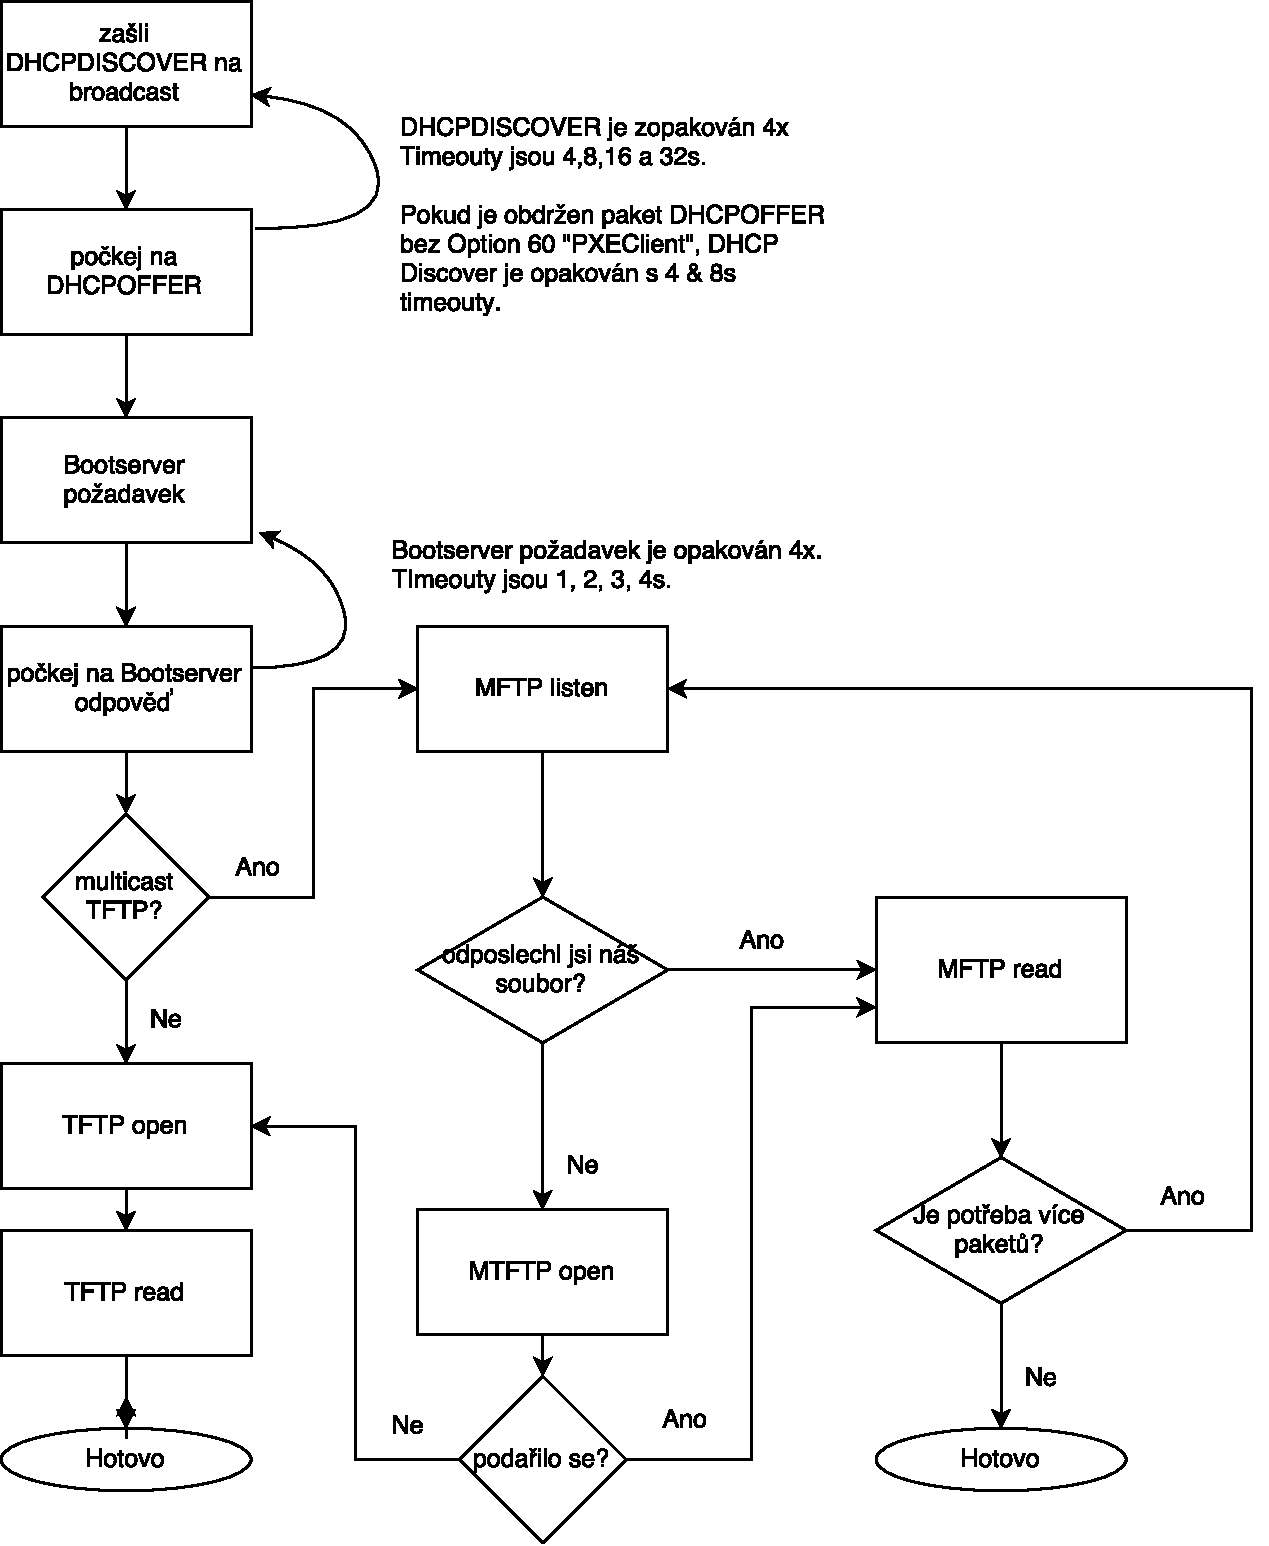
\includegraphics[width=1\textwidth]{files/pxe-flow.pdf}
	\caption{Diagram popisující průběh dle PXE}\label{fig:float}
\end{figure}

\begin{enumerate}

\item  Klient zahájí komunikaci zasláním DHCPDISCOVER paketu na broadcast adresu. K~tomu se využije standartního portu DHCP - 67 na UDP. Tento paket obsahuje rozšíření, podle kterého server pozná, že paket příchází od klienta s~implementovaným PXE protokolem. Konkrétně tedy DHCP Option 60, nastavena na PXEClient:Arch:xxxxx:UNDI:yyyzzz. (Předpokládáme, že DHCP server toto rozšíření podporuje.)

\item  Odpoví na standardním DHCP reply portu (UDP 68) paketem DHCPOFFER. Každá zpráva obsahuje klasické DHCP parametry - IP adresu klienta a další možnosti nastavené administrátorem serveru.

\item Z~DHCPOFFER paketu si klient zaznamená:
\begin{itemize}
\item IP adresu klienta,
\item seznam Boot serverů z~PXE tagu,
\item Discovery Control Options,
\item IP adresu Multicast Discovery.

\end{itemize}

\item  Pokud si klient vybere IP adresu nabídnutou DHCP službou, pak musí dokončit standartní DHCP průběh zasláním požadavku na adresu (paketu DHCPREQUEST) a poté počkáním na potvrzení požadavku od služby -- obdržením paketu DHCPACK.

\item  klient si vybere a objeví Boot server. Tento objevovací paket může být zaslán na broadcast (port 67), multicast (port 4011) nebo na unicast (port 4011). Toto záleží na nastavení obdržené v~předchozím přijatém DHCPOFFER paketu obsahující rozšiřující PXE tagy. Paket je stejný jako počáteční DHCPDISCOVER v~kroku 1, jen je organizován jako DHCPREQUEST a obsahuje:

\begin{itemize}
\item IP adresu přiřazenou klientovi z~DHCP,
\item tag pro identifikátor klienta (UUID),
\item tag pro klientovo UNDI,
\item tag pro klientovu achitekturu serveru,
\item DHCP Option 60 - nastavenou na PXEClient:Arch:xxxxx:UNDI:yyyzzz.
\end{itemize}

\item  Boot server vyšle na unicast klientovi paket DHCPACK na klientův zdrojový port. Tento paket obsahuje:

\begin{itemize}
\item jméno zaváděcího souboru
\item konfigurační parametry MTFTP \footnote{Multicast Trivial File Transfer Protocol}
\end{itemize}

\item  Klient stáhne spustitelný soubor buď pomocí standardního TFTP (port 69), nebo MTFTP (potom přiřazený port nalezneme v~Bootserver ACK paketu). Kam se server uloží, záleží na architektuře procesoru klienta.
\item  Klient rozhodne, zda je potřebný test staženého souboru. Pokud je test zapotřebí, klient zašle další DHCPREQUEST boot serveru požadující identifikační údaje staženého souboru. Tyto identifikační údaje stáhne a provede test, zda je soubor správný.

\item  Konečně, pokud podmínka kroku 8 proběhla pozitivně, PXE klient začne vykonávat kód právě staženého souboru.
\end{enumerate}

\section{Zavaděč operačního systému}

Pomocí výše uvedené série kroků do počítače chceme nahrát určitý kód. Tím kódem je zavaděč systému -- pro naše využití bylo využito bootloaderu pxelinux (patřící do kolekce zavaděčů syslinux). Zavaděčem nazýváme krátký kód, uložený v~tabulce MBR \footnote{Master Boot Record}, nebo boot sektoru jednoho z~oddílů disku. Účelem zavaděče je, aby do operační paměti počítače nakopíroval další, větší program -- tím je např. jádro operačního systému. Následně přeskočí na zkopírovaný kód a tím mu předá řízení počítače.


Zavaděče lze rozdělit do dvou kategoríí \cite{syslinux-abc}:
\begin{enumerate}

\item na primární (first-stage) -- jsou přímo obsaženy na hardware počítače. Na IBM-kompatibilních PC se tento zavaděč nazývá BIOS,
\item a sekundární (second-stage), které jsou zavolány primárním zavaděčem. Mezi ně patří právě syslinux, nebo dobře známý GRUB \cite{grub}.
\end{enumerate}

\subsection{Syslinux (pxelinux)}

V~porovnání s~GRUB je syslinux velmi jednoduchým zavaděčem \cite{syslinux-grub-comparsion}. Ve skutečnosti syslinux je kolekcí zavaděčů, každý zavaděč pro jiný účel:

\begin{enumerate}

\item syslinux je určen  pro bootování ze souborového systému FAT,
\item isolinux, pro bootování z~ISO 9660 filesystému, který je používán na CD,
\item pxelinux je určen pro bootování ze síťového serveru (tedy naše řešení),
\item extlinux -- bootování ze souborového systému ext2/ext3.
\end{enumerate}

\section{Automatizace instalace linuxových distribucí}

Následující sekce popisuje způsoby instalace linuxových distribucí bez interakce člověka. Bohužel tento proces pro všechny distribuce nebyl unifikován. Je tedy nutné použít více instalátorů v~jednom prostředí. Příští strany se budou věnovat instalátorům pro operační systémy Debian (instalátor pod názvem Preseed) a Red Hat Enterprise Linux (Kickstart).
%\subsection{Instalační skripty}

%Na různých linuxových distribucích můžeme balíčkové manažery kombinovat. Bohužel prvotní instalace - a také nástroj, pomocí kterého tento proces vykonáváme, je specifický ke každé distribuci . Pokud tedy budeme chtít provozovat heterogenní prostředí, s velikou pravděpodobností se nevyhneme použití několika instalátorů vedle sebe. Následující podkapitoly

\subsubsection{Automatizace instalace OS Debian pomocí Preseed}

\label{preseed}

Při instalaci operačního systému Debian a distribucí na něm založených, preseeding (pozn. v~překladu do češtiny přednastavení) nám umožňuje odpovědět na otázky při instalaci OS, které bychom jinak byli nuceni vyplnit ručně. Díky tomu můžeme plně automatizovat většinu instalací. Preseeding dokonce obsahuje nějaké funkce, které přes manuální instalaci nejsou dostupné. Celá tato konfigurace je obsah skriptu předložený instalaci. Následující odstavce ukazují, jak skript může být předložen a co by měl obsahovat.

\paragraph{Způsoby preseedingu}

Existují tři metody, jak skript instalaci předložit. Těmi jsou: initrd, soubor a předložení po síti.

\begin{itemize}
\item \mintinline{latex}{initrd} --  preseed konfiguraci předáme instalaci už v~ram disku; načtení skriptu se provede hned na začátku instalace. Můžeme přeskočit všechny otázky. Podmínkou je soubor \mintinline{latex}{preseed.cfg} uložený v~kořeni initrd.
\item \mintinline{latex}{soubor} -- v~tomto případě je konfigurace uložena na bootovacím médiu (tj. CD nebo USB flash disk). Načtení skriptu se provede hned po připojení média, tj. hned po dotazech na direktivy (otázky) o~jazyku instalace a rozvržení klávesnice.
\item \mintinline{latex}{ze sítě} --  načtení preseed skriptu proběhne hned po automatické konfiguraci síťových rozhraní. Boot parametr obsahující řetězec, odkud je soubor stažen, se nazývá \mintinline{latex}{preseed/url=http://server/preseed.cfg}.
\end{itemize}


V~případě této bakalářské práce je využito třetí možnosti, tj. stažení konfiguračního souboru pomocí HTTP protokolu. I~když načítání preseed konfigurace z~initrd se zdá jako nejzajímavější způsob, generování initrd instalátoru je poměrně komplexní proces.


\paragraph{Preseed soubor}

Preseed soubor je plain text soubor, ve kterém každý řádek obsahuje jednu odpověď na jednu \mintinline{latex}{debconf} direktivu. Jeden řádek obsahuje čtyři pole oddělené mezerou (nebo tabulátorem). Na příkladu
\begin{minted}{bash}
d-i mirror/suite string stable
\end{minted}
\begin{itemize}

\item \mintinline{latex}{d-i} -- první pole je tzv. vlastník direktivy; \uv{\mintinline{latex}{d-i}} je značka pro direktivy spojené s~instalátorem,
\item \mintinline{latex}{mirror/suite} je identifikátor a typ otázky oddělené lomítkem,
\item \mintinline{latex}{string stable} jsou jsou datový typ a hodnota odpovědi. Pokud řádek obsahuje další mezeru, považuje se za část odpovědi.
\end{itemize}




\subsubsection{Automatizace instalace CentOS/RHEL pomocí Kickstart}

\label{kickstart}
Kickstart je způsob automatizované instalace od společnosti RedHat. Kvůli této vazbě je tedy kompatibilní s~operačnímy systémy vázanými na tuto společnost, jmenovitě Red Hat Enterprise Linux (zkráceně RHEL), CentOS, Fedora.

Základem Kickstart instalace jsou tři prvky: malý bootovací obraz disku, konfigurační soubor a repozitář s~jednotlivými balíčky. Díky PXE instalaci obraz disku a kickstart soubor nemusí být  uložen na záznamovém médiu připojeném k~serveru. Kickstart nabízí širokou škálu možností, jak si instalaci přizpůsobit vlastní potřebě. Pěkným a užitečným způsobem, jak toto nastavit je jeden plain text soubor (\mintinline{latex}{ks.cfg}).

Soubor obsahuje část s~příkazy odkazující na jednotlivé kroky při instalaci. V~souboru předáme stejné parametry, které bychom provedli, pokud bychom instalovali interaktivně.

Kickstart soubor \mintinline{latex}{ks.cfg} se skládá z~těchto částí:

\begin{itemize}

\item nastavení klávesnice a jazyka operačního systému,
\item způsob autentifikace,
\item diskové rozdělení,
\item výběr bootloaderu,
\item seznam balíčků, které se na stroj budou instalovat,
\item a konečně vlastní příkazy, které se mají provést v~okamžiku, co skončí instalace (tzv. post-install skript).
\end{itemize}

Další ze zajímavých vlastností ks.cfg je částečně automatizovaná instalace, případně aktualizace. Instalátor se poté zeptá jen na otázky, které mu nebyly podsunuty v~konfiguračním souboru (mezi toto může například patřit rozdělení disku, které můžeme chtít u~každého serveru jiné). Některé možnosti aktualizace operačního systému pokmocí kickstartu jsou ale omezené -- například není možné aktualizovat verze balíčků.


\paragraph{Rozdělení disku}

Následující část pojednává o~možnostech kickstart instalace při rozdělení disků. Příkazy níže je možné vložit do konfiguračního souboru (\mintinline{latex}{ks.cfg}).

\mintinline{latex}{autopart} -- automaticky vytvoří diskové oddíly -- 1 GB a více pro root oddíl (\mintinline{latex}{/}), swap oddíl a boot oddíl podle příslušící architektury. Tento příkaz též přijímá parametry \mintinline{latex}{--encrypted} a \mintinline{latex}{--passphrase=PASS}.

\mintinline{latex}{ignoredisk} -- zapříčiní, že disk nebude využit. Parametr poté je\\ \mintinline{latex}{--drives=disk1,disk2,...} Druhým využitím příkazu je parametr\\ \mintinline{latex}{--use-only=disk1}, pomocí kterého určíme, pouze jaké disky máme použít.

\mintinline{latex}{raid} vytvoří software RAID. Struktura příkazu vypadá takto:
\begin{minted}{bash}
raid <mntpoint> --level=<level> --device=<mddevice> <partitions*>
\end{minted}

\mintinline{latex}{Mntpoint} je místo, kde bude vytvořený raidový oddíl připojen. Podmínkou je, že oddíl připojený na \mintinline{latex}{/boot} musí být RAID typu 1 (To samé platí i pro root oddíl, pokud nemáme zvláštní boot oddíl). Parametr level nám říká typ RAIDu  (0, 1, 4, 5, 6, nebo 10).

\mintinline{latex}{part / partition} -- vytvoří diskový oddíl na disku. K~zajímavým parametrům patří \mintinline{latex}{<mntpoint>}, \mintinline{latex}{--fstype} (případně \mintinline{latex}{--noformat}), \mintinline{latex}{--size}.

\mintinline{latex}{bootloader} -- specifikuje, jak by měl být bootloader instalován. Pomocí parametru \mintinline{latex}{--location} nastavíme oddíl (případně pozici Master Boot Recordu, pokud nastavíme \mintinline{latex}{--location=mbr}), kde má být záznam zapsán. Parametr \mintinline{latex}{--driveorder} říká, který disk je první v~pořadí v~nastavení BIOSu.

		\mintinline{latex}{clearpart} odstraní všechny diskové oddíly na discích specifikovaných v~parametru \mintinline{latex}{--drives}. S~pomocí \mintinline{latex}{--initlabel} vytvoříme label standardní k~naší architektuře, tedy GPT, či MBR.


\subsubsection{Disková rozvržení}

Před úspěšnému dokončení instalace operačního systému na server si musíme zodpovědět několik otázek. Před kopírováním systémových souborů musí být cílové médium (většinou hard disk) nastaveno. Nastavením je myšlena série kroků, do které patří

\begin{itemize}

\item partitioning, neboli vytvoření oddílů -- jednotlivé oddíly disků jsou části disku (ať už fyzického nebo logického), se kterými můžeme libovolně nezávisle manipulovat. Diskový oddíl obsahuje svůj vlastní souborový systém, připadně pododdíly,
\item naformátování disku, při kterém na oddíl zavedeme souborový systém,
\item vytvoření zavaděče disku,
\item nakopírování souborů na disk.
\end{itemize}


\section{Formáty diskových oddílů}


Na počítačích s~procesorem z~rodiny x86 (IBM PC kompatibilní) je proces bootování obyčejně řešen jedním ze dvou způsobů. Tím prvním a zároveň starším je BIOS-MBR, nebo novější UEFI-GPT. Následující odstavce přiblíží, jak metody fungují.

% Metoda UEFI-GPT je modernější, a proto podporuje užití většího počtu diskový oddílů, kdy jednotlivé oddíly můžou mít i větší velikost. V porovnaní s BIOS-MBR zvyšuje též rychlost a bezpečnost bootování.

\subsection{Standardní proces bootování s~MBR}

% http://www.pcguide.com/ref/mbsys/bios/bootSequence-c.html

MBR je starým standardem pro rozdělování oddílů disku a stále je ve velké míře používán. MBR (master boot record), se nachází na úplném začátku disku a obsahuje metadata o~tom, jak jsou na zařízení logické oddíly organizovány. Master Boot Record též obsahuje spustitelný kód, který je schopen prohledávat oddíly a najít na nich operační systém. A~následně spustit spustitelný kód/proceduru operačního systému.


Na MBR disku je možné mít pouze 4 oddíly. Pro vytvoření více oddílů je potřeba nastavit tu čtvrtou jako \uv{rozšířenou}  (tj. \uv{extended}), ve které je možné vytvořit pod-oddíly (též logické disky). Tím, že MBR využívá 32 bitů na adresu oddílu, je maximální velikost jednoho do 2TB. Takto nějak vypadá typické rozdělení MBR:
\newpage



\begin{figure}[H]\centering
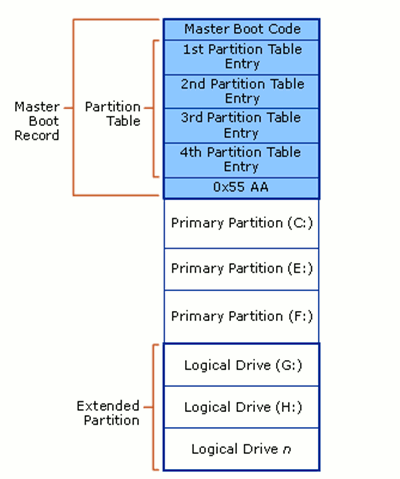
\includegraphics[width=0.5\textwidth]{files/mbr-disk-layout.png}
	\caption{MBR rozvržení disku \cite{gpt-mbr-pic}}\label{fig:float}
\end{figure}



Jak vidíme na obrázku výše, MBR má několik nevýhod. Vedle již zmíněné maximální velikosti oddílu 2TB a maximálně 4 logických oddílů, to je též fakt, že MBR je jediné místo, kde se nachází informace o~diskovém rozdělení. Pokud se tedy někdy poruší, celý disk se stane nečitelným.


% Standartní bootovací proces BIOS-MBR od zapnutí počítače po načtení operačního systému na počítačích IBM-PC kompatibilních se skládá z následujících kroků:
% \begin{itemize}
%
% \item Zapnutí počítače -- Po zapnutí či reštartu serveru sa procesoru pošle signál RESET,
%  který na sběrnicích ukončí všechny aktivity a nastaví obsah vybraných registrů na počáteční hodnoty. Procesor se potom spustí v 16b reálném módu.
% \item Spuštění BIOS kódu -- Po spuštění počítače procesor vždy nastaví obsah instrukčního ukazatele (ip – instruction pointer) na výrobcem zvolenou adresu reset vektoru
% (například pro procesor 80836 to je fyzická adresa 0xfffffff0) a začne vykonávat instrukce na nadcházejících adresách. Reset vektor ukazuje do oblasti, která obsahuje kód BIOSu. BIOS představuje firmware počítače a implementuje základní program poskytující služby na komunikaci s hardware. Jeho programový kód je uložený v ROM, EEPROM nebo flash paměti umístěné na základní desce počítače. Mezi základní úlohy BIOSu při bootovaní patří testování (POST) a inicializace hardware. Následně BIOS vyvolá přerušení int 19h.
% Vyvolaním tohoto přerušení resp. služby se BIOS na základě svojí konfigurace pokusí najít bootovací zařízení (pevný disk, CD, DVD a pod.), které obsahuje bootovací sektor. Bootovací sektor je úplně první sektor, resp. oblast velká 512 bajtů, která se nachází na CHS adrese 0/0/1 (cylinder 0, hlava 0, sektor 1) příslušného bootovacího zařízení. Aby byl tento sektor platný, musí obsahovat tzv. boot sektor podpis. To
% znamená, že bootovací sektor musí být zakončený dvojicí bajtů 0x55,
% 0xaa.
%
% Na paměťových médiích, které je možné rozdělit na více diskových
% oddílů, se první sektor nazývá master boot record (MBR). V ostatních případech, kdy bootovací sektor se nachází na oddílu, nazývame ho volume boot record (VBR). BIOS ale mezi tím nerozlišuje. Snaží se jen najít platný bootovací sektor (sektor
% s boot podpisem), jehož obsah následně přesune na předurčenou adresu do RAM paměti a předá mu řízení.
% \item Spuštění kódu MBR/VBR -- MBR resp. VBR je přesunutí do paměti RAM na fyzickou adresu 0x7c00.
% Segmentový registr cs a registr ip se nastaví tak, aby také ukazovali
% na stejnou adresu (klasicky cs = 0x0000; ip = 0x7c00). Program
% umístěný na této adrese je následně spuštěn. Ve většině případů
% MBR obsahuje krátký program -- primární zavaděč (primary bootloader),
% jehož úlohou je nalezení aktivního oddílu a následně předání
% řízení do VBR tohto oddílu. VBR většinou obsahuje kód sekundárního zavaděče, ktorý je závislý na operačním systému. Klasicky jeho
% hlavní úlohou je najít a nahrát do paměti RAM a spustit obsah sektorů,
% na kterých je umístěný soubor skutečného zavaděče operačního
% systému.
% \end{itemize}


\subsection{Standardní proces bootování s~GPT}

GPT je posledním standardem pro rozdělování oddílů na disku, současně je částí UEFI standardu. Využívá globálně unikátních identifikátorů (GUID), pomocí kterých definuje oddíl. Pro systém založený na UEFI tedy je nezbytné, aby využíval GPT. Je teoreticky možné vytvořit neomezený počet oddílů -- na většině operačních systémů je ale toto číslo omezeno na 128. Narozdíl od MBR, které je omezeno na 2TB, jeden oddíl může být velký až $ 2^{64} $ bloků (64 bit adresa). Při bloku velkém 512 bajtů je to 9.44 ZB (1 ZB je miliarda TB). Na diagramu \ref{gpt-pic} vidíme rozvržení disku s~GPT.
\newpage

\begin{figure}[h]\centering
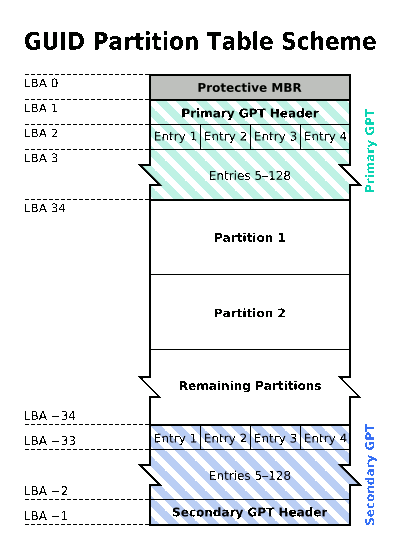
\includegraphics[width=0.5\textwidth]{files/gpt-partition-scheme.png}
	\caption{GPT rozvržení disku \cite{gpt-mbr-pic}}\label{gpt-pic}
\end{figure}

Jak ukazuje obrázek \ref{gpt-pic}, primární GPT se nachází na začátku disku a sekundární na konci. To je jedna z~funkcionalit, co dělá GPT účinnější než MBR. GPT ukládá záložní hlavičku a tabulku oddílů na konci disku, takže pokud se nějakým způsobem primární poškodí, může být zachráněna a obnovena ze sekundární. Také obsahuje CRC32 opravné součty pro detekování chyb v~hlavičce anebo tabulce oddílů. Dále můžeme vidět \uv{Protective MBR} v~prvním sektoru disku. Pomocí tohoto hybridního nastavení můžeme počítač s~biosem zavést z~disku s~GPT rozdělením, se zavaděčem uloženým v~části \uv{Protective MBR}. Tato funkcionalita je též ochranou před poškozením od nástrojů, které o~GPT neví.


\chapter{Analýza provisioning frameworků}

V~této kapitole rozeberu jednotlivé frameworky, pomocí kterých je možné nainstalovat operační systém. Jednou z~nutných podmínek je schopnost instalace operačních systémů CentOS a Debian. Ostatní operační systémy jsou výhoda, ale nejsou nezbytné. Kapitola též popisuje stroje, na kterých bude celý experiment testován spolu s~jejich konfigurací. Služby jsou konfigurovány tak, aby byly na oddělených virtuálních serverech a nemohly se vzájemně ovlivňovat. Na konci kapitoly vybereme framework Foreman z~důvodů níže uvedených.

\section{Metodika porovnání}

Než začnu zkoumání a hodnocení jednotlivých frameworků, je třeba si stanovit hodnotící kritéria, která mi umožní frameworky objektivně porovnávat a vybrat kandidáta pro kapitolu \b{Nasazení Foremanu}. Pokud to bude alespoň trochu možné, tak pro kritérium stanovím stupnici, na základě které bude možné frameworky mezi sebou porovnat.


Zhodnocení jednotlivých frameworků pro provisioning čistého hardwaru bylo provedeno jak z~pohledu kvality, tak i kvantity. Jakmile je framework nastaven a rozvržen, může být složité klientské servery zmigrovat z~jednoho na druhý. Kritéria zvolené při porovnáváni jsou následující:


\begin{itemize}
\item uzavřenost systému (licence),
\item dospělost projektu,
\item počet aktivních uživatelů,
\item složitost instalace frameworku,
\item stabilita,
\item složitost údržby,
\item hardwarová náročnost,
\item počet volitelných vlastností.
\end{itemize}

Následující podkapitoly přiblíží frameworky ke srovnání. Dále popíši jednotlivé parametry, podle kterých frameworky budeme porovnávat.



\section{Testovací laboratoř}


\subsection{Hardware}
\subsubsection{Master server}

Celý experiment byl testován na Intel x86 stroji se základní deskou X10SLM-F od výrobce SuperMicro. Na kartě je zapojen BMC modul pro vzdálené ovládání. Další fakta o~serveru jsou:

\begin{itemize}
\item Intel® Xeon® E3-1200 v3,
\item 16 GB RAM,
\item 1x 10Gbps Intel GE síťová karta,
\item 2x512 GB SSD disky zapojené jako JBOD. \footnote{Just a bunch of disks - v~překladu jen hromada disků}
\end{itemize}


\subsubsection{Instalovaný stroj}

Instalovaný stroj má tyto parametry:

\begin{itemize}
\item základní deska X10DDW-i,
\item Intel® Xeon® E3-1200 v3,
\item 16 GB RAM,
\item 1x 10Gbps Intel GE síťová karta,
\item 1x 1Gbps Intel XE síťová karta,
\item 1x 4TB HDD.
\end{itemize}

Koncept instalace serverů je navržen tak, že hlavní, tedy 10 Gbit síťová karta je zapojena do podsítě připojené do internetu. IP adresa na této síťové kartě přiřazena staticky na stroji. 1 Gbit port je zapojen do interní sítě oddělené od internetu, na které bude celý proces instalace probíhat. IP adresa je na tomto portu přiřazována pomocí DHCP. Připojení k~internetu při instalaci probíhá pomocí http-proxy, její adresa je zaslána serveru v~Kickstart/preseed konfiguračním souboru.


\subsubsection{Přepínač mezi stroji}

Jako přepínač mezi stroji byl využit Cisco SF550X-24. Na portu, na kterém je připojen master server, je povolen VLAN trunking. Pakety, které nejsou označkované (tagované), patří do VLAN 1. Na tomto portu jsou také povolené pakety otagované jako VLAN 222.

Na instalovaném stroji je konfigurace nasledující:

1Gbps síťová karta je připojena do VLAN 222 (trunkování VLAN není povoleno).
10Gbps síťová karta je připojena do VLAN 1 (trunkování VLAN není povoleno).

\subsection{Konfigurace strojů}

V~následujících podkapitolách popíši, jaká nastavení na serverech byla provedena.
\subsubsection{Master}

Na master stroji budeme všechny naše testované projekty mít v~kontejnerech. Přesněji řečeno to nebudou kontejnery, ale budeme využívat KVM (Kernel-based Virtual Machine) virtualizace, díky které můžeme jednotlivé části úplně oddělit od hypervisoru. Toto je míněho hlavně z~bezpečnostního hlediska. Jako operační systém, nad kterým budou jednotlivé služby spouštěny je vybrán Debian. Mezi důvodu patří nadstandardní stabilita, jedna z~největších komunit v~oblasti GNU/Linux a také velký výběr již vytvořených balíčků pro jakékoliv potřeby. Na síťovém portu jsou povoleny VLAN 1 a 222, přičemž pokud pokud ethernetový rámec tag s~informací o~VLANě neobsahuje, bude nastavena na 1. Tuto konfiguraci sítě pro operační systém Debian vidíme níže:

\begin{minted}{bash}
# /etc/network/interfaces
# interfaces(5) file used by ifup(8) and ifdown(8)
auto lo
iface lo inet loopback

auto br0
iface br0 inet dhcp
bridge_ports enp5s0
up /usr/sbin/brctl stp br0 off

auto enp5s0.222
iface enp5s0.222 inet static
        vlan-raw-device enp5s0

auto br1
iface br1 inet static
        address 192.168.4.4
        netmask 255.255.255.0
        bridge_ports enp5s0.222
        up /usr/sbin/brctl stp br1 on
\end{minted}

Jak vidíme výše, rozhraní br0 je VLAN 1 (dle nastavení na přepínači) a br1 je VLAN 222. Tato terminologie bude využívána i v~následujícím textu.


\section{Testované frameworky}

Kapitola níže popíše frameworky, které jsme k~naší analýze vybrali.
\section{Foreman}

Tento open source projekt spatřil světlo světa v~roce 2009, kdy byl založen programátory Ohadem Levym a Paulem Kellym. Foreman \cite{foreman} je komplexní nástroj pro správu celého životního cyklu jak hardhare strojů, tak těch virtuálních. Mezi hlavní části a funkce patří: provisioning, configurace serveru a poté jeho monitoring. Umožňuje automatizaci úkolů, které se opakují během prvotního nastavení infrastruktury. Dále Foreman nabízí správu konfigurací serverů, následovaných monitorováním a zobrazování trendů ze získaných dat.  Celý projekt je zaštítěn společností RedHat a jako jazyk byl vybrán Ruby on Rails. Databázi, do které budou ukládána data, si můžeme při instalaci vybrat -- patří mezi ně PostgreSQL, SQLite, MySQL a další. Foreman se dá také provozovat na jiných databázích, ovšem bez oficiální podpory.

Během provisioningu, Foreman z~velké části závisí na Smart Proxy, která je ve výchozím nastavení nainstalována na stejný server, jako Master uzel. Smart proxy hraje roli prostředníka v~kominikaci mezi Foremanem a externími službami. V~současnosi Smart Proxy obsahuje podporu pro služby: TFTP, DNS, DHCP, Puppet \& Puppet CA. Další služby je možné nainstalovat pomocí pluginů. Na obrázku \ref{arch-foreman} můžeme vidět komunikaci mezi Foremanem, Smart Proxy a službami.

\begin{figure}[h]\centering
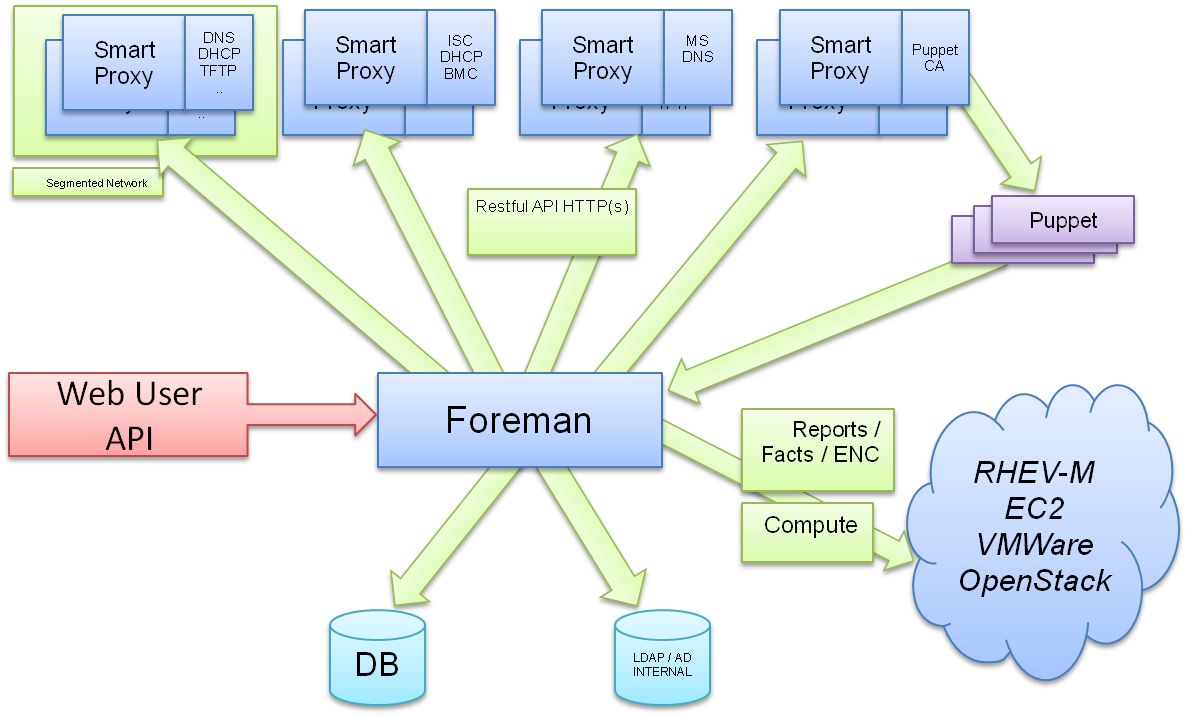
\includegraphics[width=0.8\textwidth]{files/foreman_architecture.png}
	\caption{Architektura Foremanu \cite{foreman-arch}}\label{arch-foreman}
\end{figure}


Provisioning serveru s~námi vybraným operačním systémem a požadovanou konfigurací je několika krokový proces. Prvně jě třeba vybrat operační systém s~přiřazeným instalačním médiem. Foreman již má několik operačních systémů založených na UNIXu v~sobě nakonfigurován a připraven přímo k~instalaci na stroje. Dalším krokem je vybrání rozdělení disků a šablony pro provisioning (pro příklad Kickstart nebo Preseed).

Když nainstalovaný server nabootuje pomocí PXE protokolu, vyšle broadcast zprávu pro DHCP server schopný přijímat DHCP žádosti. Smart Proxy pracující jako DHCP server odpoví a přidělí IP adresu novému hostu. PXE server je kontaktován a přesměruje nový stroj na TFTP server obsahující bootovací obraz disku. Nový stroj se pokusí o~získání obrazu, spustí ji a začne instalaci s~parametry, které byly obsažené v~šabloně ve Foremanu. Následovně, pokud je tak povoleno, proběhne jeden běh Puppetu. Foreman spoléhá na službě Puppet pro správu konfigurací a pro sbírání faktů o~serverech. Celý proces je zobrazen na obrázku \ref{foreman-arch-2}.

\begin{figure}[h]\centering
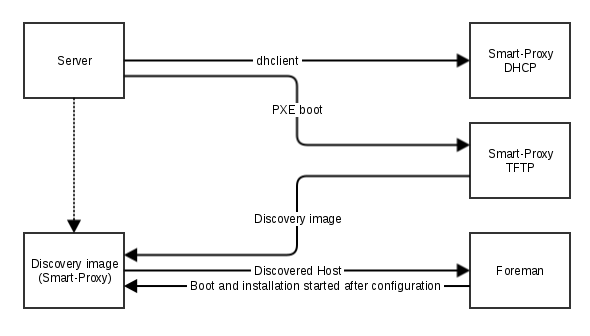
\includegraphics[width=0.8\textwidth]{files/discovery.png}
	\caption{Zavedení OS pomocí Foremanu \cite{foreman-arch2}}\label{foreman-arch-2}
\end{figure}


Foreman je schopen zavést široké spektrum operačních systémů založených na UNIXu. Mezi operační systémy, které se podle diskusních fór povedlo nainstalovat, patří: RHEL, Fedora, CentOS, Ubuntu, Debian, Solaris 8 and 10, OpenSUSE. Každopádně oficiální seznam operačních systémů, které Foreman podporuje, je poněkud kratší. Patří mezi ně: RHEL 6 and 7, CentOS 6 and 7, Fedora 19, Debian 7, Ubuntu 12.04 and 14.04 \cite{foreman-support-os}.

Foreman nabízí grafické rozhrací pro jednoduché využívání i méně schopnými uživateli. Je též dostupné RESTful API. Další variantou ovládání Foremanu je jeho nástroj pro ovládání z~příkazové řádky -- zvaný Hammer. Pomocí něj je možné jednotlivé dílčí kroky skriptovat. Foreman je jednoduše rozšiřitelný pomocí Rails Engines. To ukazuje široká škála již dostupných rozšíření. Mezi ně patří například rozšíření Azure, Digital Ocean a další - pro přímý provisioning virtuálních serverů ve zmíněných cloudech.

\subsection{Foreman Smart Proxy}

Jádrem řídícího systému Foremanu pro vzdálené části infrastruktury jsou Smart Proxy \cite{foreman-proxy}, což jsou malé a modulární aplikace vytvořené v~Ruby. Zjednodušeně, pokud něco spravovat, spustíme jednu z~těchto ruby aplikací v~místě, kde potřebujeme. Například, místo toho, abychom se manuálně připojili k~DHCP serveru, podívali se na zápůjčky IP adres, přímo se pomocí REST API DHCP serveru zeptáme na volnou IP adresu, kterou nám DHCP server vrátí. Kód těchto proxy serverů je cíleně velmi krátký -- okolo 1000 řádků, díky čemuž není tak těžké jednotlivým částem porozumět a dopsat libovolný modul.

Mezi tyto smart proxy moduly patří:
\begin{itemize}

\item DHCP, DNS, TFTP,
\item BMC/IPMI,
\item Puppet, Puppet CA,
\item MCollective \cite{mcollective}.
\end{itemize}

Foreman obsahuje koncept zvaný Compute Resources. Tento nápad cílí na provisioning virtuálních serverů (také bare metal) na veřejných a soukromých cloudech. Podporuje tedy například VMWare infrastrukturu, nebo EC2.

% Stroje ve Foremanu jsou děleny na dvě části -  managed a unmanaged. Managed stroje můžeme například restartovat, nainstalovat nový OS, atp. Unmanaged stroj je zjednodušeně jen Puppet slave (v puppet terminologii Agent), který komunikuje s naším Puppet Masterem. Unmanaged server je možné přeměnit na managed a následně ho přes grafické rozhraní ovládat. Je tedy možné do nástroje přidat ve velkém až stovky serverů, které už fungují.

% Pokud chceme vytvořit nový host (tj. provision host), ať už na bare metalu, nebo na cloudu, vybereme, kam instalovat. Pokud je stroj bare metal, námi vytvořený host a fyzický stroj v datacetru se mezi sebou matchují pomocí mac adresy.

% Provisioning Templates


% Integrace puppetu.

% Puppet je velmi silně integrován do foremanu.

\section{Razor}

Razor \cite{razor} je jednou z~aplikací pro zavedení operačního systému na bare-metal servery a virtuální systémy. Jedním z~cílů frameworku je dostání serveru do stavu, kdy aplikace pro zaslání konfgurací na server (jako jsou např. Ansible nebo Puppet) mohou převzít kontrolu.

Servery nově přidané do Razoru pomocí PXE standadu stáhnou a spustí obraz disku zvaný Razor microkernel image, který aplikaci zašle informace o~serveru a vyčká na další instrukce. Razor podle předem předpřipravených pravidel od uživatele vyhodnotí, jaký model (tj. jaký operační systém, jaké diskové rozložení, atp.) má na server aplikovat. Nový uzel začne následovat instrukce dle modelu, odpovídá Razoru a dokončí instalaci. Model může obsahovat např. instalaci Puppetu a registraci k~nějakému serveru s~běžící aplikací pro správu serverů.

\section{Stacki}

Stacki \cite{stacki} je nabízen ve dvou základních plánech. V~plánu zdarma, ten ale nenabízí webové rozhraní. Placený plán sice přes webovou stránku ovládat lze, skrývá ale v~sobě jiná omezení. Mezi tato omezení paří například nemožnost instalace distribucí založených na Debianu (tedy i Ubuntu, které je jedním z~našich požadavků), dále neobsahuje podporu pro UEFI. UEFI v~nasěm případě problém není, protože SuperMicro základní karty v~nastavení umožňují změnu na Legacy Boot (BIOS), absence podbory Debian distribucí je ale pro nás závážná, až klíčová.

\subsection{Edice zdarma}

Základní verzi Stacki můžeme nalézt zdarma, bohužel je ořezaná o~určité vlastnosti. Jednou z~možností je stažení rpm balíčku pro CentOS. Po instalaci balíčku dostaneme skript, který server přetransformuje na Stacki frontend. Druhou možností je, stejně jako u~placené verze, připraný ISO obraz pro instalaci na stroj bez operačního systému.

\subsection{Pro plán}

Placená edice Stacki softwaru je nabízena ve 14-ti denní zkušební verzi, tu jsem také pro tento experiment použil. Po registraci na webu produktu je odeslán e-mail s~odkazem na stažení iso souboru. Obraz je ve své podstatě CentOS linux (můžeme si vybrat CentOS 6, či 7) přípravený pro vypálení na CD, nebo zkopírování na USB disk pro následovné zavedení systému a instalaci na čistý stroj. Tento postup je odlišný od ostatní opensource konkurence, jež nabízejí svoje provision frameworky většinou jako balíčky pro linuxové disribuce. Cena placené edice je 100 USD/rok na jeden uzel, hlavní výhodou je již zmíněná podpora UEFI a možnost instalace Ubuntu a v~neposlední řadě placená podpora.



\section{OpenStack Ironic}

OpenStack \cite{openstack} je škálovatelná, open-source platforma pro stavbu veřejných či privátních cloudů. Jako distribuční model převažuje IaaS, česky přeloženo jako \uv{Infrastruktura jako služba}. V~takovémto modelu se poskytovatel služeb zavazje poskytnout infrastrukturu -- ať už virtualizované, tak i hardware servery. Příklady komerčních IaaS jsou např. Amazon Web Services, nebo Microsoft Azure.  OpenStack je stavěný na velké výpočetní, datové i síťové zdroje v~datacentrech, u~čehož je vě ovládáno přes webové rozhraní.

Všechny OpenStack služby mezi sebou komunikují na bázi RESTful API, k~tomuto využívají HTTP protokol pro výměnu informací a dat. Jednou komponentou je právě Ironic pro instalaci bare metal serverů.

OpenStack je orientován na obrovské clustery. Věřím, že v~určitých případech může být správnou volbou i pro provisioning, v~našem případě ale taková volba připadá jako kolos. Už jen instalace celého frameforku na jeden systém (v~mém případě vybraném DevStacku) trvala něco přes půl hodinu. Z~důvodů nevhodnosti pro naše využití jsem se s~testováním tohoto frameworku dále nezabýval.


\section{Spacewalk}


Spacewalk \cite{spacewalk} je open source nástrojem pro administraci Linux serverů. Licencí, pod kterou je distribuován, je GPLv2\cite{gpl2}. Spacewalk je software řízený komunitou, vyvinuly se z~něj ale i nějaké komerční produkty -- mezi ně patří například Red Hat Satellite \cite{satellite} nebo Novell SUSE Manager \cite{suse-manager}. Vývoje framerworku Spacewalk začal v~červnu 2008 a v~té době se oficiálně stal open-source projektem. Základem je Red Hat Network, založený v~roce 2001 -- z~tohoto projetu se později stal oddělený Red Hat Satellite produkt.

Spacewalk má mnoho vlastností umožňujících linuxovým administrátorům správu hardwaru. Umožňuje instalovat a aktualizovat systémy, konfigurovat systémy ve skupinách, zavést operační systém na bare-metal server a následně ho nastavit, včetně instalace monitorování. Spacewalk též spolupracuje s~virtualizačními platformami, jako jsou VMWare, nebo Xen \cite{xen}, na kterých vytvoří virtuální servery. Administrační software podporuje mnoho linuxových distribucé, mezi které patří např. Fedora, CentOS, SLES and Debian na architekturách 32bit, i 64bit.


\subsection{Licence}

V~této práci se budu zabývat pouze open-source frameworky, tedy pokud nějaký framework chceme zvažovat, musíme nejdříve zjistit, zda nám to licence projektu dovoluje. Licence frameworku může ovlivnit licenci díla, kde framework použijeme (tedy i tuto bakalářskou práci). Důvody pro open-source jsou zřejmé:

\item nulové počáteční náklady - získáme zdarma produkt, krerý by jinak společnost vyvíjela několik měsíců. Díky tomu je ušetřeno na počátečních nákladech,
\item bezpečnost - oprava 0 Day \cite{0day} zranitelností a dalších chyb je díky komunitě skoro okamžítá,
\item žádné proprietární uzamčení a lepší kvalita kódu.

Licence se dají rozdělit podle stupně přísnosti. Níže uvedené rozdělení je od nejméně přísného až po nejstriktnější:

\begin{itemize}
\item Public Domain,
\item permisivní,
\item LGPL,
\item copyleft,
\item AGPL.
\end{itemize}

Všechny analyzované frameworky se nacházejí pod určitou open-source licencí, nebo alespoň mají ekvivalentní open-source edici. OpenStack Ironic, Foreman, Cobbler i MaaS jsou kompletně open-source a zdarma.


\begin{table}[h]
\centering
\caption{Frameworky: License}
\label{Frameworky_licence}
\begin{tabular}{lllllll}
\toprule
 Foreman & Ironic & Razor & Stacki & Spacewalk & Cobbler \\ \midrule
 GNU GPL 3    &  Apache &  Apache &  BSD, placená   &   GNU GPL 2  & GNU GPL 2
\end{tabular}
\end{table}




\subsection{Stáří projektu}

\uv{Nedospělý}, či netestovaný kód, který se může jednoduše rozbít, přímo koreluje se stářím frameworku. Je proto důležité se ujistit, že projekt, který vybereme bude použitelný a dospělý.  V~naší analýze je dospělost spočítána pomocí počtu let, jak dlouho je framework vyvíjen.

Počet uživatelů či počet nasazení systému nám může ukázat určité náznaky, jako jaká je populárnost systému u~určité společnosti a které důvody se za tím skrývají. Tato hodnota, aby byla přesná, není jednoduše zjistitelná. Určité metriky jsou ale veřejně dostupné -- mezi ty patří například počet forků na GitHubu, počet uživatelů v~mailing listu, počet velkých firem, které se rozhodly pro nasazení frameworku (zde vycházím z~předpokladu, že ve velké společnosti tým na takový úkol bude mít větší počet pracovníků a tím i přispěvatelů do projektu). Tyto hodnoty nám můžou nastínit určitý odhad, kolik nasazení bylo. Toto nám také v~určité míře ukazuje, jaká rychlost bude při opravách různých chyb, či rychlost přidávání dalších funkcí.



\begin{table}[h]
\centering
\caption{Frameworky: Stáří projektu}
\label{Frameworky_oldness}
\begin{tabular}{lllllll}
\toprule

 Foreman & Ironic & Razor & Stacki & Spacewalk & Cobbler \\ \midrule
  2009        & 2013       &  2013     & 2015       &  2008         & 2011
\end{tabular}
\end{table}

\begin{table}[h]
\centering
\caption{Frameworky: počet forků na GitHubu}
\label{Frameworky_oldness}
\begin{tabular}{lllllll}
\toprule

 Foreman & Ironic & Razor & Stacki & Spacewalk & Cobbler \\ \midrule
  598        & 188       &  139     & 25       &  127         & 402
\end{tabular}
\end{table}


%
% \subsection{Složitost instalace}
%
% Dalších z hlavních bodů, které musíme při výběru frameworku zvažovat, je složitost instalace takovéhoto systému pro provizi serverů. Jedním
%
% \subsection{Stabilita}
%

\subsection{Složitost užití}

Všechny analyzované frameworky mají webové grafické rozhraní, pomocí kterého je možné servery provizovat. Díky tomu by měla být uživatelská přívětivost na slušné úrovni. Výjimkou je Razor, u~kterého je grafické rozhraní pouze placené verzi (tj. Puppet Enterprise). Objevil jsem grafické rozhraní \cite{puppet-dashboard}, které by zmíněný problém mělo vyřešit, není ale součástí analýzy.

\subsection{HW požadavky}

Dříve, než začneme instalovat jakýkoliv software, musíme se ujistit, zda hadware, na který program chceme nainstalovat, je dostatečný. I~přes to, že hardware dostupný pro experiment se zdál dostatečný, v~případě instalace Ironic nestačil. Pro jeho provozování je třeba sestavit celý cluster -- pro experiment tedy místo OpenStacku byl vybrán DevStack \cite{devstack}, který bohužel svojí rychlostí neoslnil. Všechny ostatní frameworky s~poskytnutým výpočetním výkonem a pamětí problém neměly.


\subsection{Podpora discovery}

Je důležité, aby vybraný framework podporoval tzv. discovery -- tedy objevení a zjištění základních informací o~serverech, které které jsou nové a ještě v~databázi nejsou. Většina frameworků má tuto funkcionalitu vytvořenou způsobem linuxové image, která se načte místo operačního systému na neznámých strojích. Tento malý linux si poté pokusí nastavit připojení k~síti, DNS, a pokud se zdaří, odešle frameworku zpět informace o~novém serveru. Mezi informace může patřit například počet procesorů, velikost paměti, nebo typ síťové karty. Ve frameworku Foreman se tato funkcionalita nazývá Discovery \cite{foreman-discovery}, v~Razoru zase EL Microkernel \cite{el-microkernel}. Tabulka \ref{Frameworky_discovery} ukazuje, zda testovaný nástroj objevování nových strojů podporuje.



\begin{table}[h]
\centering
\caption{Frameworky: Podpora funkcionality discovery}
\label{Frameworky_discovery}
\begin{tabular}{lllllll}
\toprule

- & Foreman & Ironic & Razor & Stacki & Spacewalk & Cobbler \\ \midrule
  & ANO        &  ANO      &  ANO     & ANO       &  ANO         & NE
\end{tabular}
\end{table}


\subsection{Podpora operačních systémů}

Jedním z~prvních požadavků bylo, že daný framework bude podporovat instalaci různých operačních systémů (alespoň linuxových distribucí). Například MaaS podporuje pouze Ubuntu -- je vydáván společností Canonical (společnost zaštitující Ubuntu). Proto mnoho funkcionalit MaaS je již zakomponováno do Ubuntu. Cobbler i Ironic mají podporu instalace pouze linuxových distribucí. Foreman zvládne jak různé linuxové distrubuce, tak BSD systémy, i Windows. Podporu Windows s~určitými úravami má také Razor. Framework Stacki je stavěn předně pro linuxovou distribuci CentOS (v~oficiální podpoře), Debian a Ubuntu pouze s~komunitní podporou. V~tabulce \ref{Frameworky_os} jsou vidět frameworky a jejich podporu instalovaných operačních systémů:



\begin{table}[h]
\centering
\caption{Frameworky: Podpora operačních systémů}
\label{Frameworky_os}
\begin{tabular}{lllllll}
\toprule

 Foreman & Ironic & Razor & Stacki & Spacewalk & Cobbler \\ \midrule
 Linux        & Linux       & Linux      & Linux       & Linux          & Linux \\
 Windows         &        & Windows      &        &           &

\end{tabular}
\end{table}




\section{Závěr}


V~této kapitole popíši a shrnu jednotlvé frameworky v~jejich silných i slabých bodech podle poznatků, které jsem získal při testování systémů a podle posbíraných statistických dat.


\subsection{Foreman}



Z~výše testovaných frameworků po analýze byl vybrán Foreman. Hlavní výhodou bylo jeho grafické rozhraní, pomocí kterého může administrátor vykonat reinstalaci serveru na jakémkoliv zařízení s~webovým prohlížečem. To samé se týká i serverového technika, který je schopen práci vykonat na svém telefonu, stojící vedle serveru v~serverovně. Jeho instalace byla v~porovnání s~ostatními frameworky stejně obtížná, z~důvodu, že implicitní konfigurace není ideální a je třeba systém hluboce nastudovat, pokud ho nevyužíváte na uživatelské úrovni. Výhodou jsou již vytvořené balíčky pro master server, Smart Proxy, i nějaké pluginy do operačního systému Debian, což konkurence v~podobě Spacewalk, Stacki a dalších nenabízí. Mezi další důvody mého výběru Foremanu patří jedna z~největších komunit v~této oblasti a také časté vydávání nových verzí. Nasazením frameworku se věnuje příští kapitola.


\subsection{Ostatní frameworky}


V~této části práce následuje přehledná tabulka popisující, jak si frameworky v~jednotivých kategoriích vedly. Podrobnější tabulky o~každém kritériu byly uvedeny v~příslušných sekcích.
\newpage
\begin{table}[H]
\centering
\caption{Srovnání frameworků}
\label{srovnani-frameworku}
\rotatebox{90}{

\begin{tabular}{@{}l|llllll@{}}
\toprule

metrika &	Foreman & Ironic & Razor & Stacki & Spacewalk & Cobbler  \\ \midrule
Uzavřenost systému &  GNU GPL 3    &  Apache &  Apache &  BSD, placená   &   GNU GPL 2  & GNU GPL 2 \\
Dospělost projektu &   2009        & 2013       &  2013     & 2015       &  2008         & 2011 \\
Počet forků na GitHubu & 598        & 188       &  139     & 25       &  127         & 402 \\
Intalované OS & Linux        & Linux       & Linux      & Linux       & Linux          & Linux \\
& Windows         &        & Windows      &        &           & \\
Podpora discovery & ANO        &  ANO      &  ANO     & ANO       &  ANO         & NE \\
%Počet aktivních uživatelů & & & & & & \\
% Složitost instalace frameworku & & & & &  & \\
% Stabilita & & & & &  & \\
% Složitost údržby & & & & & &  \\
% Podpora discovery  & & & & &  & \\
% Hardwarová náročnost & & & & &  & \\
% Počet features & & & & &  & \\ \bottomrule
\end{tabular}
}
\end{table}

\begin{table}[h]
\centering
\caption{Informace o~frameworcích}
\label{my-label}
\begin{tabular}{@{}lll@{}}
\toprule

Framework &	Webová stránka &	Testovaná verze  \\ \midrule
Foreman & https://www.theforeman.org/ & 1.14.3 \\
Ironic & https://wiki.openstack.org/wiki/Ironic & 1:5.1.2-0ubuntu1  \\
Razor & https://github.com/puppetlabs/razor-server & 1.7.0 \\
Stacki & https://github.com/StackIQ/stacki & 4.0  \\
Spacewalk & https://spacewalk.redhat.com/ &  2.6 \\
Cobbler & http://cobbler.github.io/ & 2.8.0  \\  \bottomrule
\end{tabular}
\end{table}
\newpage

Tabulka výše ukazuje verze frameworků testované v~této analýze spolu s~odkazy na domácí stránky projektů.

\chapter{Nasazení Foremanu}

Cílem této kapitoly je popsání nasazení frameworku Foreman, který jsme vybrali v~minulé kapitole. V~první části popíši topologii infrastruktury. Dále budou postupně popsány jednotilivé servery a služby, které na nich běží. Na konci kapitoly je popsán Ansible a jeho playbooky, pomocí kterých je možné infrastrukturu jednoduše nasadit.

\section{Topologie infrastruktury}

Jedním ze stavebních kamenů virtualizace je vymezení běhu operačního systému do virtualizovaného prostředí, přičemž jsou mu poskytnuty částečné či plné zdroje virtualizačním nástrojem. Díky tomu můžeme na jednom fyzickém stroji provozovat více virtuálních počítačů. Dává nám to možnost lépe a efektivněji využít výpočetního výkonu stroje (tzv. hypervisoru) s~dalšími výhodami, mezi které patří např. možnost hostování více operačních systémů na jednom serveru.
Výhodou virtualizovaných prostředí je dozajista oddělenost a jednoduché znovunasazení instancí. V~našem případě budeme jednotlivé části infrastuktury virtualizovat pomocí KVM.


\subsection{KVM}


KVM je virtualizační infrastruktura pro linuxové jádro, které ho přemění na hypervisor. Aplikaci začala vyvíjet společnost Qumranet, později odkoupená RedHatem. V~linuxovém kernelu je obsaženo od verze 2.6.20. Podporovaná je pouze plná virtualizace, plnou virtualizací ale lze spouštět i proprietární operační systémy, jako macOS, Windows, Solaris. Ke své funkčnosti vyžaduje nejméně podporu virtualizace procesoru první generace a to buď procesory od společnosti AMD pod označením AMD-VTM(1) či od společnosti Intel s~registrovanou ochranou známkou IntelR VT.



\begin{figure}[h]\centering
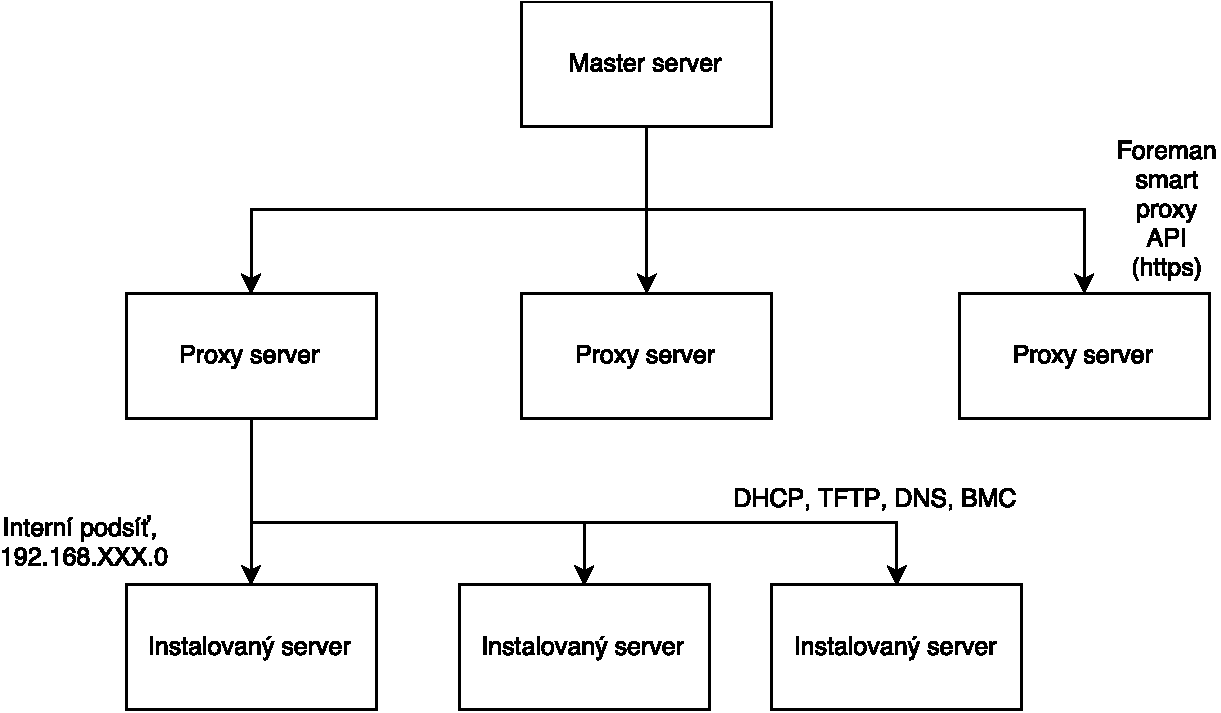
\includegraphics[width=1\textwidth]{files/infrastruktura-v2.pdf}
	\caption{Infrastruktura}\label{fig:float}
\end{figure}


\section{Master server}

Master server je instalován na operačním systému Debian, na serveru virtualizovaném pomocí infrastruktury KVM. Hlavní službou je nástroj Foreman, jehož instalace je dále popsána.

\subsection{Foreman}

Před samotnou instalací je třeba přidat repozitáře pro balíčkovací utilitu apt-get, jelikož verze chtěných aplikací nemusí být v~oficiálních repozitářích aktuální.

\begin{minted}{bash}
echo "deb http://deb.theforeman.org/ jessie 1.14"
    > /etc/apt/sources.list.d/foreman.list
echo "deb http://deb.theforeman.org/ plugins 1.14"
    >> /etc/apt/sources.list.d/foreman.list
apt-get -y install ca-certificates
wget -q https://deb.theforeman.org/pubkey.gpg -O- | apt-key add -
\end{minted}

Poté co jsou přidány repozitáře je možné nainstalovat  \mintinline{latex}{foreman-installer}.

\begin{minted}{bash}
apt-get update && apt-get -y install foreman-installer
\end{minted}

Instalátor je možné spustit buď v~interaktivním módu, kdy je uživatel dotázán na nastavení na obrazovce. Druhou možností je vyplnění konfiguračního souboru \mintinline{latex}{/etc/foreman-installer/scenarios.d/foreman-answers.yaml}, ze kterého si instalátor sebere odpovědi automaticky. V~příloze práce je tento soubor vyplněn. (Vytvořen jako šablona v~Ansible).


V~interaktivním módu je vygenerováno heslo pro uživatele admin, pomocí kterého je možné se přihlásit do uživatelského webového rozhraní. Pokud použijeme Ansible z~přílohy práce, je třeba toto heslo v~konfiguračním souboru \mintinline{latex}{defaults/defaults.yaml} upravit a to bude aplikováno.


\subsubsection{Disková rozdělení}

V~teoretické části práce byly popsány výhody a nevýhody formátování oddílů disku pomocí MBR či GPT. V~instalovaných serverech touto infrastrukturou se bude používat MBR pro malé disky (do 1TB) a to z~důvodu kompatibility základních desek. Při větších kapacitách již využijeme GPT rozdělení z~důvodů popsaných v~teoretické části práce.

Práce obsahuje šablony pro operační systémy Debian a CentOS (a operační systémy z~nich odvozené) a to pro:
\begin{table}[]
\centering
\caption{Podpora diskových rozdělení}
\label{gptnmbr}
\begin{tabular}{lll}
        & Kickstart  & Preseed    \\
NO RAID & GPT \& MBR & GPT \& MBR \\
RAID1   & GPT \& MBR & GPT \& MBR \\
RAID0   & GPT \& MBR & GPT \& MBR
\end{tabular}
\end{table}


\subsection{Zálohování}

V~případě této práce je v~konfiguraci užita relační databáze PostgreSQL. V~databázi jsou uloženy  informace o~serverech, statistiky a metadata Foremanu. Díky tomu, že krátký čas odstávky vadit nebude, je možné si dovolit udělat zálohu databáze metodou dump. Obecně dump je soubor, který obsahuje strukturu tabulek a dále data obsažená v~těchto tabulkách. Dle rady v~manuálu \cite{foreman-backup} dále zálohujeme adresáře

\begin{itemize}
\item \mintinline{latex}{/etc/foreman} obsahující všechny konfigurační soubory Master Foremanu
\item \mintinline{latex}{/var/lib/puppet/ssl} -- obsahující certifikáty
\end{itemize}

Celé zálohování blíže popisuje shellový skript uložený v~\\\mintinline{latex}{/usr/local/bin/foreman-backup.sh}:
\begin{minted}{text}
#!/usr/bin/env bash

# Backup The Foreman, following the advice at
# http://theforeman.org/manuals/1.7/index.html#5.5.1Backup

set -e # If any command fails, stop this script.
ME=$(basename $0)
main () {

  DATE=$(date '+%Y%m%d.%H%M')
  BACKUPDIR=/data/backups/backup-$DATE
  mkdir $BACKUPDIR
  chgrp postgres $BACKUPDIR
  chmod g+w $BACKUPDIR

  cd $BACKUPDIR

  # Backup postgres database
  su - postgres -c "pg_dump -Fc foreman > $BACKUPDIR/foreman.dump"

  # Backup config ifles

  tar --selinux -czf $BACKUPDIR/etc_foreman_dir.tar.gz
      /etc/foreman
  tar --selinux -czf $BACKUPDIR/var_lib_puppet_dir.tar.gz
      /var/lib/puppet/ssl
  tar --selinux -czf $BACKUPDIR/tftpboot-dhcp.tar.gz
      /var/lib/tftpboot /etc/dhcp/ /var/lib/dhcpd/

  ls -lh *tar.gz foreman.dump

}

main 2>&1 | /usr/bin/logger -t $ME
\end{minted}

Tento skript je spouštěn každý den ve 2 hodiny ráno. Opakované spouštění je řešeno pro UNIX klasickým způsobem, tedy pomocí CRON démona. Řádek v~CRON tabulce pro uživatele root (otevřeme pomocí příkazu \mintinline{latex}{crontab -e}) vypadá následovně:

\begin{minted}{text}
2 0 * * *  /usr/local/bin/foreman-backup.sh
\end{minted}



Následovně ještě celý filesystem serveru zálohujeme pomocí utility backuppc \cite{backuppc}. Jediné co je pro klienta potřebné spustit, je rsync v~démon módu. Nainstalujeme tedy rsync a vytvoříme služby pro systemd.

Je potřeba vytvořit soubor  \mintinline{latex}{/etc/systemd/system/rsyncd.socket} s~obsahem:
\begin{minted}{text}
[Unit]
Description=Rsync Server Activation Socket
ConditionPathExists=/etc/rsyncd.conf

[Socket]
ListenStream=873
Accept=true

[Install]
WantedBy=sockets.target
\end{minted}

Soubor se systemd službou, nacházející se v~\\\mintinline{latex}{/etc/systemd/system/rsyncd@.service}:

\begin{minted}{text}
[Unit]
Description=Rsync Server
After=local-fs.target
ConditionPathExists=/etc/rsyncd.conf

[Service]
# Note: this requires /etc/rsyncd.conf
ExecStart=/usr/bin/rsync --daemon
StandardInput=socket
\end{minted}



Dříve, než můžeme tuto službu použít, je ještě potřeba vytvořit soubor \mintinline{latex}{/etc/rsyncd.conf}. V~nejjednodušší konfiguraci bude obsahovat:

\begin{minted}{text}
lock file = /var/run/rsync.lock
log file = /var/log/rsyncd.log
pid file = /var/run/rsyncd.pid

[foreman]
    path = /home/foreman
    uid = rsync
    gid = rsync
    read only = no
    list = yes
    auth users = rsyncclient
    secrets file = /etc/rsyncd.secrets
    hosts allow = 192.168.1.0/255.255.255.0
\end{minted}


Soubor \mintinline{latex}{/etc/rsyncd.secrets} obsahuje uživatelská jména a hesla oddělená dvojtečkou. Následovně je třeba nastavit na souboru správná přístupová práva, aby ostatní uživatelé nebyli schopni soubor číst, či nijak upravovat.
\begin{minted}{text}
# chmod 600 /etc/rsyncd.secrets
\end{minted}


\subsection{Zabezpečení serveru}

Jedním z~prvků zabezpečení je nastavení firewallu na serveru. Protože používáme operační systém Debian, jako firewall máme k~dispozici iptables. Na serveru zakážeme všechny porty mimo:

\begin{table}[h]
\centering
\caption{Otevřené porty na hlavním uzlu}
\label{my-label}
\begin{tabular}{@{}lllll@{}}
\toprule

Port &	Protokol &	Potřebné pro  \\ \midrule
53 &	TCP \& UDP &	DNS Server \\
67, 68 &	UDP &	DHCP  Server \\
69 &	UDP	&  TFTP Server \\
 443 &	TCP HTTP\/S &  Foreman UI a provisioning templates \\
3000 &	TCP	HTTP &  Foreman UI a provisioning templates \\
3306 &	TCP &	v~případě oddělené PostgreSQL databáze \\
5910 - 5930 &	TCP &	Server VNC Consoles \\
5432 &	TCP &	v~případě oddělené PostgreSQL databáze \\
8140 &	TCP &	Puppet Master \\
8443 &	TCP &	Smart Proxy, otevřená pouze pro Foreman \\ \bottomrule
\end{tabular}
\end{table}

\label{lets-encrypt}
Dalším krokem je vynucení SSL při připojení do webového rozhraní Foremanu. V~posledních letech byl představen projekt Let's Encrypt pod záštitou neziskové instituce Internet Security Research Group (ISRG). Let's Encrypt otevřená certifikační autorita (CA), nabízející digitální certrifikáty potřebné k~HTTPS (SSL/TLS) zdarma.

V~našem případě, kdy pro frontend využíváme webový server Apache (httpd) je vytvoření a obnova certifikátu velmi jednoduchá. Před vygenerováním certifikátu je nutné nastavit DNS A~záznam tak, aby mířil na IP adresu přiřazenou našemu serveru. Tento A~záznam musí být stejný jako hostname nastavený na serveru.  Postup instalace certifikátu a jeho obnovení je následovný:

Nainstalujeme balíček s~názvem certbot:

\begin{minted}{text}
# apt-get install python-certbot-apache
\end{minted}

Aktuálně už můžeme certbot klient použít. Vygenerování SSL certifikátu pro Apache je poměrně přímočaré. Klient automaticky získá a nainstaluje nový SSL certifikát pro validní domény v~Apache konfiguraci.

Interaktivní instalaci certifikátů vyvoláme pomocí příkazu:

\begin{minted}{text}
# certbot --apache
\end{minted}


Certbot projde získanou Apache konfiguraci a najde domény, které by měli být v~žádosti o~certifikát obsaženy. Interaktivně je možné jakoukoliv doménu odebrat. Utilita se dotáže na email potřebný při ztrátě klíče a dá nám na výběr ze dvou možností:

\begin{itemize}
\item povolený http a https přístup, pokud je nějaká potřeba pro nezašifrovanou komunikaci,
\item nebo přesměrování z~http na https, které my využijeme.
\end{itemize}

Když instalace proběhne, vytvořené certifikáty spolu se soukromým klíčem jsou k~dispozici v~adresáři \mintinline{latex}{/etc/letsencrypt/live}.

Zda je certifikát validní je možné zjistit například pomocí následujícího odkazu:

\begin{minted}{text}
https://www.ssllabs.com/ssltest/analyze.html?d=example.com\&latest
\end{minted}

Certifikáty vydávané autoritou Let's Encrypt jsou validní na 90 dní, proto je potřeba je po uplynulé době obnovovat. Doporučená doba k~tomu je 60 dní. Aplikace ertbot obsahuje parametr renew, pomocí kterého certifikát obnovíme.

Praktickým způsobem, jak na linuxovém stroji vykonávat nějakou činnost opakovaně, je cron démon. Protože obnovovací příkaz zjišťuje pouze datum expirace a obnoví certifikát pouze pokud do expirace zbývá méně, než 30 dní, není problém tuto činnost spustit například jednou týdně.

Úpravu CRON tabulky uživatele root provedeme následovně:

\begin{minted}{text}
# crontab -e
\end{minted}

Příkaz otevřel soubor \mintinline{latex}{/var/spool/cron/crontabs} pomocí našeho editoru. Do souboru přidáme řádek a uložíme:

\begin{minted}{bash}
30 2 * * 1 /usr/bin/certbot renew >> /var/log/le-renew.log
\end{minted}

Tato část automaticky spustí aplikaci \mintinline{latex}{/usr/bin/certbot renew} každé pondělí ve dvě ráno, v~době, kdy by server neměl být tak těžce zatížen. Informace o~průběhu se uloží do logu v~adresáři \mintinline{latex}{/var/log}.


\section{Proxy server}




\subsection{Nastavení sítě}
\label{proxy-network}
Tento virtuální server má přístup ke dvoum odděleným sítím. První z~nich je připojena do internetu (toto síťové rozhraní nazvěme eth0) a má IP adresu přiřazenou z~veřejného rozsahu. Adresa je nastavena staticky na stroji. Druhá síť je interní. Na tomto proxy serveru adresu přiřadíme staticky, u~dalších strojů se adresa přiřadí pomocí DHCP (DHCP server bude spuštěn na tomto serveru).


Zde definujeme rozsah sítě pro každou lokalitu:

\begin{minted}{text}
10.22.X.0/24,
\end{minted}

kde X je číslo lokality, ve které se proxy server nachází. Maska podsítě \mintinline{latex}{/24} nám říká, že síť bude schopna obsáhnout 255 počítačů. Proxy server v~lokalitě č. 1 tedy bude mít vlastní adresu \mintinline{latex}{10.22.1.1/24}.

\subsection{Foreman Smart Proxy}

Smart Proxy je projektem nabízejícím restové API jednotlivým subsystémům. Je tedy rozhraním mezi automatizačními nástroji vyšší úrovně (např. Foreman) a službami nižší úrovně (jako je DHCP, DNS, TFTP, atd.).

Pro instalaci balíčku v~operačním systému Debian je třeba přidat repozitáře Foremanu z~adresy \mintinline{latex}{deb.theforeman.org}. \cite{fproxy-install} Postup přidání repozitářů je stejný jako u~master serveru, proto zde není popsán. Poté nainstalujeme balíček pomocí \mintinline{latex}{apt-get} a aplikaci nastavíme. Jednou z~klíčových částí konfigurace je nastavení komunikace s~Foreman master serverem pomocí SSL. Toto je blíže popsáno v~kapitole Zabezpečení serveru.
\subsection{konfigurace DHCP}


Smart proxy potřebuje pro svou funkci správně fungující PXE stack, do kterého patří i DHCP server. Osobně jsem využil serveru od ISC, kvůli obrovské uživatelské podpoře a celkové vyladěnosti. V~repozitářích Debianu lze nalézt pod jménem \mintinline{latex}{isc-dhcp-server}. Ukázková konfigurace je níže:

\begin{minted}{text}
omapi-port 7911;
max-lease-time 86400;

option domain-name-servers 8.8.8.8;

allow booting;
allow bootp;

option fqdn.no-client-update    on;  # set the "O" and "S" flag bits
option fqdn.rcode2            255;
option pxegrub code 150 = text ;

# PXE Handoff.
next-server SERVER_IP;
filename "pxelinux.0";

log-facility local7;

include "/etc/dhcp/dhcpd.hosts";

subnet 192.168.2.0 netmask 255.255.255.0 {
range 192.168.2.10 192.168.2.255;
  option subnet-mask 255.255.255.0;
  option routers SERVER_IP;
\end{minted}


Výše vidíme nakonfigurované direktivy. Lease time (čas propůjčky IP adresy) můžeme nastavit libovolně. Povolení bootp a booting direktiv je nutná podmínka k~funkčnosti PXE. Řádka \mintinline{latex}{filename "pxelinux.0"}; značí soubor, který bude instalovanému stroji podsunut. Lokace souboru na proxy serveru je v~adresáři \mintinline{latex}{/var/lib/tftpboot}. Implicitně se soubor nachází v~adresáři \mintinline{latex}{/usr/share/syslinux/}, odkud je možné ho přesunout. Též je třeba, aby adresář obsahoval soubor \mintinline{latex}{menu.c32}. Nastavení podsítě je znovu libovolné, zde nastaveno podle kapitoly \ref{proxy-network}. Proměnná \mintinline{latex}{SERVER_IP} obsahuje IP adresu Smart Proxy.



\subsection{konfigurace TFTP}

Pro nastavení TFTP serveru využiji balíčku xinetd. Jeho nastavení je poměrně triviální; konfigurace TFTP se nachází v~adresáři \mintinline{latex}{/etc/xinetd.d/tftp}:
\begin{minted}{bash}
service tftp
{
 protocol = udp
 port = 69
 bind = SERVER-IP-BIND
 socket_type = dgram
 wait = yes
 user = nobody
 server = /usr/sbin/in.tftpd
 server_args = /srv/tftp
 disable = no
}
\end{minted}


\subsection{Zabezpečení serveru}

Komunikaci mezi Smart proxy a hlavním uzlem vykonáváme přes zabezpečené spojení SSL. Prvním krokem k~tomu je vytvoření certifikátu podepsaným Master serverem. Na hlavním uzlu tedy vykonáme příkaz (parameter SERVER-HOSTNAME je FQDN \footnote{Fully Qualified Domain Name; FQDN přesně určuje umístění počítače ve stromové struktuře DNS.} nově vytvořeného proxy serveru):


\begin{minted}{text}
$ /opt/puppetlabs/bin/puppet cert --generate SERVER-HOSTNAME
\end{minted}

Výstupem příkazu jsou 3 soubory:
\begin{itemize}
\item certifikát nově vytvořené proxy
\item soukromý klíč nově vytvořené proxy
\item certifikát hlavního uzlu
\end{itemize}

Tyto soubory přesuneme na proxy server a po změníme čtecí práva pouze pro uživatele foreman-proxy.

Druhým bodem zabezpečení serveru je firewall. Stejně jako na hlavním uzlu máme operační systém Debian, použijeme tedy iptables.

Povolené porty jsou následující:

\begin{table}[h]
\centering
\caption{Otevřené porty na proxy serveru}
\label{open-ports}
\begin{tabular}{@{}lllll@{}}
\toprule

Port &	Protokol &	Potřebné pro  \\ \midrule
53 &	TCP \& UDP &	DNS Server \\
67, 68 &	UDP &	DHCP  Server \\
69 &	UDP &  TFTP Server \\
5910 - 5930 &	TCP &	Server VNC Consoles \\
8140 &	TCP &	Puppet Master \\
8443 &	TCP &	Smart Proxy, otevřená pouze pro Foreman \\ \bottomrule
\end{tabular}
\end{table}
  % has broken table


\section{Collectd plugin}

Cílem našeho rozšíření je mít v~grafickém rozhraní systému Foreman jednoduché grafy, které zobrazují informace o~nainstalovaných serverech. Mezi tyto informace patří například vytížení procesoru, využití paměti, nebo přenos dat na síťovém rozhraní. Takových systémů na sběr dat existují stovky, proto v~rozsahu bakalářské práce nemá smysl vyvíjet další. Na pomoc jsem si vzal démon na sběr statistických dat, collectd. Nabízí mnoho doplňků, díky kterým můžeme o~serverech sbírat skoro jaékoliv informace nás napadnou.

\subsubsection{bootstrap na nově instalovaných serverech}

Na serverech, které jsou přes foreman instalovány se po prvotní provizi operačního systému nainstaluje collectd a poté nakonfiguruje v~klient režimu. V~příloze je skript, který collectd nastaví následovně:

\begin{minted}{bash}
	LoadPlugin contextswitch
	LoadPlugin cpu
	LoadPlugin df
	LoadPlugin disk
	LoadPlugin entropy
	LoadPlugin interface
	LoadPlugin load
	LoadPlugin memory
	LoadPlugin processes
	LoadPlugin uptime
	LoadPlugin users
	LoadPlugin vmem
	LoadPlugin tcpconns

	<Plugin df>
	  FSType "rootfs"
	  IgnoreSelected true
	  ReportInodes true
	</Plugin>
	LoadPlugin network
	  <Plugin network>
	  ReportStats true
	    <Server "ctd-server-ip" >
	      SecurityLevel "Encrypt"
	      Username "username"
	      Password password
	    </Server>
	</Plugin>
\end{minted}

V~této chvíli jsou již metriky (ty, co jsou vybrané mezi načtenými pluginy) odesílány na server s~IP adresou server-ip.

% TODO: skript, co ziska z API passw a pak si ho ulozi.


\subsubsection{server s~uloženými daty}

Všechna statistická data jsou uložena na dalším odděleném serveru. Tento počítač ma dle předchozí kapitoly IP adresu "ctd-server-ip". Aplikace collectd zde běží v~server režimu a naslouchá na portu 0.0.0.0:25826 na UDP. Tomu napovídá níže přiložená konfigurace v~collectd.conf:

\begin{minted}{bash}
Hostname FIXME-HOSTNAME
FQDNLookup false
Interval 30
ReadThreads 1
LoadPlugin syslog
<Plugin syslog>
        LogLevel info
</Plugin>
LoadPlugin rrdtool
LoadPlugin network

## Server config
<Plugin network>
  Listen "0.0.0.0" "25826"
  ReportStats true
	SecurityLevel "Sign"
  AuthFile "/etc/collectd/auth_file"
</Plugin>

<Plugin rrdtool>
        DataDir "/var/lib/collectd/rrd"
</Plugin>
\end{minted}

Jak můžeme vidět, uživatelská jména a hesla jsou ukládána do souboru /etc/collectd/auth\_file. Konfigurační soubor má formát

\begin{minted}{bash}
username1: pass1
username2: pass2
\end{minted}

% TODO: skript, který přidá řádek pro každý username ve foremanovi + vygeneruje heslo

% TODO: skript rest api, které pro danou IP vrátí uname + ip

\subsubsection{Collectd Graph Panel}

Pro poskytnutí grafů na serveru s~uloženými daty využijeme vynikajícího projektu Collectd Graph Panel. Tento grafický frontend je vytvořený v~jazyce PHP a distribuovaný pod licencí GPL 3. Pro instalaci potřebujeme nainstalovaný \mintinline{latex}{rrdtool}, který je možné operačním systému Debian získat následovně:
\begin{minted}{text}
# apt-get install rrdtool
\end{minted}





Dále webový server s~podporou PHP verze alespoň 5.0, použijeme tedy nám známý Apache server (httpd) s~pro nás postačujícím \mintinline{latex}{mod_php}.

\begin{minted}{text}
# apt-get install apache2 libapache2-mod-php

# a2enmod mod_php
\end{minted}


Instalace Collectd Graph Panelu je velmi jednoduchá. Vezmeme oficiální git repozitář, který naklonujeme do \mintinline{latex}{DocumentRootu} webového serveru.

\begin{minted}{text}
$ git clone https://github.com/pommi/CGP
\end{minted}

V~této podobě již CGP zobrazuje grafy. Pro naše potřeby je ale nutné ještě nakonfigurovat zabezpečené připojení na webovém serveru a omezit přístup do aplikace pouze z~určitých IP adres. Před nastavením zabezpečeného připojení potřebujeme povolit ssl modul v~Apache web serveru:
\begin{minted}{text}
# a2enmod ssl
\end{minted}

Získání certifikátu od certifikační autority Let's Encrypt je popsáno na straně \pageref{lets-encrypt}.


% Dalším krokem je vytvoření self-signed certifikátu. Nástrojem pro to bude OpenSSL, konkrétně nástroj v příkazové řádce pro vytváření certifikátů, klíčů, žádostí, atp:
% \begin{minted}{bash}

% openssl req -x509 -nodes -days 365 -newkey rsa:2048 -keyout /etc/apache2/ssl/apache.key -out /etc/apache2/ssl/apache.crt
% \end{minted}

% Zde popíši, co jednotlivé přepínače dělají.


% \begin{itemize}

% \item req je "podpříkaz" pro management X.509 certifikačních žádostí. V kryptografii je X.509 standard pro systémy založené na PKI (veřejném klíči).
% \item -x509 tento přepínač nám říká, že chceme vytvořit self-signed certifikát místo vygenerování certifikační žádosti.

% \item -nodes nám speciikuje, že nechceme zapezpečit náš klíč pomocí slovního hesla. Pokud bychom tak udělali, Apache by nebyl schopný se sám spustit a museli bychom zadat heslo vždy, když webserver nastartuje.

% \item  -days 365 nám říká, že certifikát bude platný pro příští rok.
% \item -newkey rsa:2048 nám ve stejnou chvíli vytvoří certifikační žádost a nový soukromý klíč. Parametr "rsa:2048" řekne OpenSSL, aby vygeneroval RSA klíč s délkou 2048 bitů.
% \item -keyout je název souboru s privátním klíčem
% \item -out je jmého souboru certifikátu.
% \end{itemize}


% Dalším krokem je získání certifikátu. Pro to využijeme certifikační autority Lets Encrypt. Lets Encrypt je schopen vydávat certifikáty podepsané autoritou IdentTrust, díky čemuž jsou přijímané všemi hlavními prohlížeči.


% získání certifikátu

% Let’s Encrypt validuje
% https://www.upcloud.com/support/install-lets-encrypt-apache/






\subsection{Vývoj pluginu}


\subsubsection{Název}
Dle doporučení v~dokumentaci Foremanu má název začínat předponou "foreman\_", pro lepší identifikaci a asociaci pluginu s~projektem. Dále pokud je název víceslovný, jednotlivá slova oddělujeme podtržítkem. Protože jsou pluginy publikovány jako gemy na stránce rubygems.org, je také potřeba zjistit, zna námi zvolené jméno je stále volné (tomu pomůže i zmíněný prefix).

Námi zvolené jméno je tedy "foreman\_colletctd\_graphs".

\subsubsection{Příprava prostředí}

Na GitHubu projektu je již fungující ukázkový plugin, který je možné využít pro jakékoliv naše potřeby. Obsahuje mnoho typů chování, které je nám libo využít - mezi ně patří přidání nových modelů, přepisování pohledů, přídávání uživatelských práv, položek do menu, atp. Soubor README v~ukázce obsahuje seznam aktuálního chování.

Se základními znalostmi programu git si projekt naklonujeme na lokální stroj, kde budeme projekt vyvíjet:
\begin{minted}{text}

$ git clone https://github.com/theforeman/foreman_plugin_template
 		foreman_colletctd_graphs
\end{minted}

Tímto stáhneme aktuální verzi z~master větve do adresáře foreman\_colletctd\_graphs. Repozitář obsahuje skript na změnu jména na námi zvolené, to provedeme následovně:
\begin{minted}{text}

$ ./rename.rb foreman_colletctd_graphs
\end{minted}




\subsubsection{Instalace pluginu}

Instalace pluginu ve vývojovém prostředí je jednodužším řešením, protože kód náčítá za běhu a nené potřeba instalovat plugin jako gem. Vytvořením vývojové instance Foremanu jsme se zabývali v~kapitole ZZ.

Plugin je možné rovnou spustit (a prozkoumat jeho chování) úpravou souboru \mintinline{latex}{Gemfile.local.rb}. Také je možné vytvořit soubor \\\mintinline{latex}{foreman_colletctd_graphs.rb} v~adresáři \mintinline{latex}{bundler.d} a vložit do něj tento řádek:

\begin{minted}{bash}
# Gemfile.local.rb
gem 'foreman_colletctd_graphs',
 		:path => 'path_to/foreman_colletctd_graphs'
\end{minted}

Potom instalujeme "preface" bundle příkazem:
\begin{minted}{text}
$ bundle install
\end{minted}

A~znovu restartujeme Foreman. Nový plugin můžeme vidět v~záložce plugin tab na About Page.

\subsubsection{Vývoj}

Prvně upravíme soubor \mintinline{latex}{foreman_colletctd_graphs.gemspec} a do něj vložíme meta informace, jako jméno pluginu, autora, web stránku projektu, verzi. Dále do souboru \mintinline{latex}{lib/foreman_colletctd_graphs/engine.rb} vložíme následující:

\begin{minted}{bash}

# lib/foreman_colletctd_graphs/engine.rb
initializer 'foreman_colletctd_graphs.register_plugin',
 		:before => :finisher_hook do |app|
  Foreman::Plugin.register :foreman_colletctd_graphs do
    # the code of our plugin
  end
end
\end{minted}



% \subsubsection{Struktura pluginu}
%
% The project is a Rails::Engine [27] as described in the instructions for Foreman plugins
% in the official documentation [54]. The most adequate choice was an engine with a
% semi-isolated namespace [46], since I wanted to avoid namespace pollution resulting in
% name conflicts but I needed an access to the classes in Foreman and Katello. The plugin
% has a standard Rails project structure with minor modifications mirroring the conventions
% in Foreman and Katello projects.
\subsubsection{Deface}

Pro úpravu HTML stránek, do kterých budeme vkládat grafy, použijeme knihovnu Deface. Umožňuje nám upravit HTML pohledy bez zásahu do spodního Ruby pohledu. Použití knihovny je možné dvěma způsoby, já zde popíši jen jeden z~nich. Pro více informací je dostupná dokumentace zde \cite{deface}.


\subsubsection{Content Security Policy}

\mintinline{latex}{Content-Security-Policy} je HTTP hlavička vytvořená s~hlavním cílem snížení XSS rizik deklarováním, jaký obsah je povolen k~načtení. V~současnosti hlavičku podporují prohlížeče Google Chrome (od verze 25+), Firefox (31+), Safari (7+), i Microsoft Edge.

Ve frameworku Foreman je tato hlavička vynucena -- pomocí gemu Secure Headers. Pokud grafy vygenerované z~rrd souborů chceme načítat z~jiného serveru, do konfigurace pluginu je třeba přidat adresu serveru s~uloženými daty. Konfigurace se provádí v~souboru \\\mintinline{latex}{/usr/share/foreman/config/initializers/secure_headers.rb} a to následovně:



% \begin{figure}[h]\centering
% 
\includegraphics[width=1\textwidth]{files/truthiestmeme.jpg}
% 	\caption{Zásada programování}\label{fig:float}
% \end{figure}




%
%
% \subsubsection{Vytvoření Gemu}
%
% http://bundler.io/v1.12/guides/creating_gem.html
%
%
% \subsubsection{Balíček pro OS Debian}
%
% https://softwareengineering.stackexchange.com/questions/195633/good-approaches-for-packaging-php-web-applications-for-debian
%



\subsection{Nasazení pluginu}

V~produkčním prostředí je nasazení pluginu velmi jednoduché. Náš vytvořený .deb balíček pomocí rsync/scp technologie přesuneme na server. V~adresáři obsahující balíček napíšeme:
\begin{minted}{bash}

$ rsync -avh foreman_colletctd_graphs.deb $UNAME@$SERVERNAME:
\end{minted}

a následovně nainstalujeme nástrojem standartně obsaženým v~Debianu:
\begin{minted}{text}

$ dpkg -i foreman_colletctd_graphs.deb
\end{minted}

Dalším krokem je restartovat Foreman server, pokud máme systemd jako náš init systém, tento krok vykonáme následovně:
\begin{minted}{text}
# systemctl restart foreman.service
\end{minted}

V~této chvíli plugin máme aktivní a funkční.

\subsection{Závěr}

Ačkoliv výsledný plugin neobsahuje hodně kódu, veškerá jeho funkcionalita dle zadání je naplněna. Na obrázku v~příloze je možné vidět aktuální podobu.

Po naprogramování práce jsem objevil již vytvořený plugin foreman-colly \cite{foreman-colly}, též generující grafy sbírané démonem collectd, ale fungující na odlišném způsobu. Doplněk od Lukáše Zapletala aktivně naslouchá paketům s~metrikami, můj plugin pouze zobrazuje již vygenerované grafy. Výhledově by bylo možné tyto dvě funcionality spojit do jednoho většího doplňku.


\section{Ansible}

Ansible je nástroj určený k~automatickému nastavení strojů podle předem určených parametrů. Součástí bakalářské práce jsou konfigurační soubory pro Ansible, tzv. playbooky, pomocí kterých je možné jednotlivé části infrastruktury nakonfigurovat během několika minut.

Ansible v~porovnání s~konkurenčními nástroji, jako je např. Chef nebo Puppet, nevyžaduje žádnou instalaci agenta na koncových zařízeních. Pro připojení ke koncovým
zařízením  se tak nejčastěji používá SSH (Secure Shell). V~terminologii Ansiblu se tato zařízení označují jako uzly (angl. nodes). Informace o~jednotlivých uzlech jsou uvedeny v~inventáři (angl. Inventory), kde je možné definovat parametr uzlů.


\subsection{Inventář}

Důležitým souborem v~Ansible je tzv. Inventář (Inventory), který obsahuje informace o~nastavovaných uzlech. Formát souboru je INI \cite{ini-fmt}, kde by měly být specifikovány jména uzlů, jejich IP adresy, uživatelská jména, hesla, porty, na kterých se chceme připojit, atp. Soubor nám umožňuje jednotlivé servery seskupovat.

\begin{minted}{text}
$ cat servers_list
[master]
host1  ip_addr=10.10.1.2

[proxy]
host2  ip_addr=10.10.2.2
host3  ip_addr=10.10.3.3

[collectd]
host4  ip_addr=10.10.1.3
\end{minted}

Pro přidání další lokality do infrastruktury je tedy nutné pouze přidat server s~jeho IP adresou do Inventářového souboru (je nutné mít v~novém proxy serveru SSH klíč Ansible serveru). Při vytváření (úpravě) inventářového souboru je třeba dbát na určité požadavky:

\begin{itemize}
\item server označený jako master musí být pouze jeden,
\item collectd server též pouze jeden,
\item proxy serverů může být libovolně (role proxy musí být zprovozněna alespoň na jednom serveru -- klidně na stejném, jako master, nebo jiném).
\end{itemize}


\subsection{Spouštění příkazů v~Ansible}

Při použití Ansible jsou možné dva různé způsoby vzdáleného spuštění příkazů na nastavovaných serverech. První metodou je tzv. Ad-Hoc \cite{ansible-ad-hoc}. Tímto způsobem je možné interaktivně (z~příkazové řádky) spustit příkaz a okamžitě vidět výsledek činnosti. Příkladem je ping modul, pomocí kterého je možné zjistit, zda servery jsou po síti dostupné:

\begin{minted}{text}
$ ansible -m ping -u deployer servers_list
\end{minted}

Po vykonání příkazu Ansible s~pomocí ping modulu vyzkouší všechny servery definované v~inventářovém souboru \mintinline{latex}{servers_list}, zda jsou dostupné k~připojení přes SSH. Případem užití je většinou rychlé nasazení oprav na více serverů najednou. Těchto modulů je v~současnosti přes 500 \cite{ansible-num-modules} a s~každým vydáním nové verze jich přibývá.


Jiným přístupem při definování serverů je konfigurace pomocí Ansible Playbooků. Playbooky jsou skripty psané v~jazyce YAML. Viz krátká ukázka:
\begin{minted}{text}

---
- name : Install and configure foreman
    hosts : servers_list
    remote_user : user
    sudo : yes

  tasks :
  - name : ( os = Debian ) Install Foreman
    apt: name=foreman state=present update_cache=yes
    sudo: yes

\end{minted}


Při vykonávání Playbooku se Ansible pokusí vytvořit SSH připojení se všemi servery definovanými v~souboru \mintinline{latex}{servers_list}. Pokud konfigurovaný server obsahuje OS Debian, nainstaluje se z~repozitářů balíček Foreman. Playbooky v~příloze práce jsou složitější.

\subsection{Playbook pro Foreman a proxy servery}

Scénáře Ansiblu mohou být velice strukturovatelné. V~našem případě je rozdělíme do více souborů, a poté je budeme ovládat nadřazeným scénářem. Tato volba by měla pomoci udržet scénáře přehledné. Vytvoříme tedy role -- sady příkazů pro provedení určitých změn. Role jsou reprezentovány adresářem v~adresáři roles. Inspirací pro konfigurační soubory v~příloze bakalářské práce jsou již vytvořené playbooky pro instalaci instancí Foremanu od společnosti Adfinis Sysgroup \cite{foreman-ansible-playbooks}, volně dostupné v~jejich GitHub repozitáři.

Playbooky obsahují několik rolí, které lze na cílový server nainstalovat:


\begin{itemize}
\item Foreman pomocí Foreman instalátoru,
\item dodatečná konfigurace Foremanu (webserver, šablony obsažené ve Foremanu, instalace pluginu),
\item nastavení isc-dhcp-server,
\item nastavení TFTP serveru,
\item foreman-proxy,
\item nastavení collectd serveru pro sběr metrik.
\end{itemize}

Před spuštěním playbooku je třeba splnit určité požadavky. Pokud požadavky nejsou splněny, instalace nemusí být zakončena správně. Mezi tyto nároky patří:

Master server:

\begin{itemize}
\item správně nastavené FQDN (DNS A~záznam musí mířit na tento server),
\item vypnutý SELinux,
\item jelikož je s~Foremanem instalován i puppet, je třeba, aby stroj měl alespoň 2GB RAM paměti,
\item ve firewallu je třeba, aby porty 67, 69, 80, 443 (a další dle kapitoly Zabezpečení serveru) byly otevřené,
\item byl na konfigurovaném serveru přístup k~internetu a repozitářům Debianu.

Na proxy serveru se předpokládá, že síťové rozhraní eth0 je použito pro veřejnou síť, eth1 pro interní síť.


Playbooky jsou dostupné jak na CD práce, tak v~mém GitHub repozitáři \cite{thesis-ansible}.

%\section{Zkušenosti v~reálném provozu}





\begin{conclusion}

Úkolem této bakalářské práce bylo seznámení se s~instalací bare-metal serverů. Po seznámení se s~jednotlivými standardy, bylo třeba analyzovat frameworky, které jsou pro tuto činnost určené. Z~nich poté jeden nejvíce vyhovující vybrat, splňující: podpora grafického prostředí (a to nejlépe webové), možnost pomocí něj instalovat alespoň operační systémy Debian a CentOS. Do zadání patřilo jeden vybraný framework nasadit a do něj vytvořit plugin zobrazující grafy ze zdroje collectd.

Mezi analyzované frameworky patřily: Foreman, Openstack Ironic, Razor, Stacki, Spacewalk a Cobbler. Jako kritéria jsem mimo jiné vybral open-source licence, složitost používání a administrace, stáří projektu a podpora discovery. Kritéria nejlépe splnil framework Foreman, který je nejenom nejdéle vyvíjený, s~největší komunitou, ale dle mého uvážení také obsahuje nejpřívětivější uživatelské rozhraní.

Foreman byl poté nasazen na produkční prostředí a aktuálně je pomocí něj nainstalováno okolo 1000 serverů. V~infrastruktuře jako takové se větší problémy nevyskytly, pouze jsou třeba úpravy při přidávání strojů s~novými základními deskami, či při přidání nových operačních systémů. Dle zadání práce byl naprogramován plugin, jehož prostředí je možné vidět v~příloze. Funkčnosti bylo docíleno s~pomocí projektu Collectd Graph Panel, odkud plugin grafy získává. Plugin splnil veškeré očekávání a je stále v~infrastruktuře nasazen. Pro jednoduchost nasazení práce též obsahuje konfigurační skripty pro nástroj Ansible.

Zpracování této bakalářské práce pro mě mělo velký přínos. Velmi mi prohloubilo pochopení protokolů jako DHCP, TFTP a dalších v~PXE standardu. Získání zkušeností s~nástrojem Ansible je také velmi důležité, jelikož je v dalších projektech využiji. Jako další rozšíření této práce může být například instalace operačního systému Windows nebo již zmíněné propojení pluginu z~práce s~rozšířením foreman-colly.

%Cílem této bakalářské práce bylo prvně analyzovat frameworky pro instalaci bare metal serverů a následně vybrat jeden, který splňuje požadavky. Dále tento framework s~úpravami nasadit.  Mezi počáteční kritéria výběru mimo jiné patřilo, aby vybraný produkt byl open-source. Na základě analýz byl vybrán framework Foreman, protože měl oproti konkurenci vyčnívající uživatelské rozhraní přístupné přes webový prohlížeč. Podpora operačních systémů, které přes něj lze instalovat, byla také jedna z~nejširších -- podporuje instalaci linuxových distribucí jako OS Debian a CentOS (což bylo naší počáteční podmínkou), Arch Linux, distribucí založených na BSD a s~úpravami také instalace OS Windows.

%Další kapitola práce se věnovala nasazení frameworku Foreman vybraného v~předchozí části. Součástí nasazení bylo vytvoření šablon pro operační systémy využívající instalátor kickstart (tedy CentOS a linuxové distribuce na něm založené) a instalátor Preseed (Debian, Ubuntu a distribuce na nich sestavené). Práce tedy obsahuje šablony pro vytvoření diskových rozložení GPT a MBR, a to oboje pro disky bez RAID technologie, RAID1 a RAID0.

%Práce též obsahuje plugin do grafického rozhraní Foremanu, který bude zobrazovat grafy získané z~démonu collectd. Tohoto bylo docíleno s~pomocí projektu Collectd Graph Panel, odkud plugin grafy získává. V~práci je popsáno, jak infrastrukturu pro funkční plugin sestavit. Plugin je dostupný téže jako open-source pod licencí GNU-GPL s~odkazem v~literatuře.

%Pro jednoduché sestavení celé infrastruktury práce také obsahuje konfigurační skripty, tzv. playbooky pro nástroj Ansible. Zpracování této bakalářské práce pro mě mělo velký přínos. Velmi mi prohloubilo pochopení protokolů jako DHCP, TFTP a dalších v~PXE standardu. Získání zkušeností s~nástrojem Ansible je také velmi důležité, které v~dalších projektech využiji.

\end{conclusion}


\bibliographystyle{csn690}
\bibliography{mybibliographyfile}
\begin{thebibliography}{9}

\bibitem{bootp-rfc}
RFC 951 -- Bootstrap Protocol. Online, Duben 2017. Dostupné z~\url{https://tools.ietf.org/html/rfc951}.

\bibitem{pxe-spec}
	Berners-Lee T., Fielding R. \& Frystyk H.
	 (zobrazeno 11.12.2016.) Pre-boot execution environment (PXE) specification version 2.1. Tech. rep.
	URL: \url{ftp://download.intel.com/design/archives/wfm/downloads/pxespec.pdf}.

\bibitem{tftp-rfc}
RFC 783 -- TFTP Protocol (revision 2). Online, Duben 2017. Dostupné z~\url{https://tools.ietf.org/html/rfc783}.

\bibitem{gpl3}
The GNU General Public License v3.0 - GNU Project - Free Software Foundation. Online, Duben 2017. Dostupné z~\url{https://www.gnu.org/licenses/gpl-3.0.en.html}.

\bibitem{fproxy-install}
Installation instructions -- Smart Proxy -- Foreman. Online, Duben 2017. Dostupné z~\url{http://projects.theforeman.org/projects/smart-proxy/wiki/Installation\_{}instructions}.

\bibitem{foreman-backup}
Foreman :: Manual. Online, Duben 2017. Dostupné z~\url{http://theforeman.org/manuals/1.7/index.html#5.5.1Backup}.

\bibitem{foreman-arch}
Foreman :: Manual. Online, Duben 2017. Dostupné z~\url{http://theforeman.org/manuals/1.7/index.html}.



\bibitem{foreman-plugin}
PRAŽÁK, Ondřej. Foreman plugin for Jenkins CI. Brno, 2015. Master’s thesis. Brno University of Technology, Faculty of Information Technology. Supervisor Grác Marek.

\bibitem{framework-analysis}

A~Comparative Study of Baremetal Provisioning Frameworks \url{http://www.pdl.cmu.edu/PDL-FTP/associated/CMU-PDL-14-109.pdf}

\bibitem{ansible-modules}

ŠAMALÍK, Adam. Extension of OpenStack Modules for Ansible Platform. Brno, 2016. Bachelor’s thesis. Brno University of Technology, Faculty of Information Technology. Supervisor Hruška Martin.

\bibitem{ansible-playbooks}

Intro to Playbooks &mdash; Ansible Documentation. Online, Duben 2017. Dostupné z~\url{http://docs.ansible.com/ansible/playbooks_intro.html}.


\bibitem{foreman-ansible-playbooks}
GitHub -- adfinis-sygroup/foreman-ansible: Ansible playbook to deploy a complete Foreman instance within minutes.. Online, Duben 2017. Dostupné z~\url{https://github.com/adfinis-sygroup/foreman-ansible}.


\bibitem{ini-fmt}
INI file -- Wikipedia. Online, Duben 2017. Dostupné z~\url{https://en.wikipedia.org/wiki/INI_file}.


\bibitem{foreman-colly}
GitHub -- lzap/foreman\_{}colly: Foreman plugin for collectd. Online, Duben 2017. Dostupné z~\url{https://github.com/lzap/foreman_colly}.

\bibitem{backuppc}
BackupPC: Open Source Backup to disk. Online, Duben 2017. Dostupné z~\url{http://backuppc.sourceforge.net/}.

\bibitem{deface}
GitHub -- spree/deface: Rails 3 plugin that allows you to customize ERB views in a Rails application without editing the underlying view.. Online, Duben 2017. Dostupné z~\url{https://github.com/spree/deface}.

\bibitem{0day}
Zero-day (computing) - Wikipedia. Online, Duben 2017. Dostupné z~\url{https://en.wikipedia.org/wiki/Zero-day_(computing)}.

\bibitem{opensource}
Bad Economy Is Good for Open Source. Online, Duben 2017. Dostupné z~\url{http://www.cmswire.com/cms/web-cms/bad-economy-is-good-for-open-source-004187.php}.




\bibitem{spacewalk-replacement}
Spacewalk still a viable option? : linuxadmin. Online, Duben 2017. Dostupné z~\url{https://www.reddit.com/r/linuxadmin/comments/5muwsl/spacewalk_still_a_viable_option/}.


\bibitem{foreman-vs-puppet}
Foreman vs Puppet. Online, Duben 2017. Dostupné z~\url{https://www.upguard.com/articles/foreman-vs.-puppet}.

\bibitem{razor-install}
Installation · puppetlabs/razor-server Wiki · GitHub. Online, Duben 2017. Dostupné z~\url{https://github.com/puppetlabs/razor-server/wiki/Installation#installing-packages}.


\bibitem{puppet-gui-comparsion}
Puppet Management GUI Comparison | OlinData. Online, Duben 2017. Dostupné z~\url{https://www.olindata.com/en/blog/2014/01/puppet-management-gui-comparison}.

\bibitem{puppet-dashboard}
GitHub -- sodabrew/puppet-dashboard: The Puppet Dashboard is a web interface providing node classification and reporting features for Puppet, an open source system configuration management tool. Online, Duben 2017. Dostupné z~\url{https://github.com/sodabrew/puppet-dashboard}.


\bibitem{syslinux-abc}

LiveCD -- 1 (úvod, isolinux). Online, Duben 2017. Dostupné z~\url{http://www.abclinuxu.cz/clanky/system/livecd-1-uvod-isolinux}.

\bibitem{syslinux-grub-comparsion}
grub2 -- What is the difference between GRUB and SYSLINUX? -- Ask Ubuntu. Online, Duben 2017. Dostupné z~\url{https://askubuntu.com/questions/651902/what-is-the-difference-between-grub-and-syslinux}.


\bibitem{el-microkernel}
GitHub -- puppetlabs/razor-el-mk: The discovery kernel for razor-server. Online, Duben 2017. Dostupné z~\url{https://github.com/puppetlabs/razor-el-mk}.


\bibitem{foreman-discovery}
Foreman :: Plugin Manuals. Online, Duben 2017. Dostupné z~\url{https://theforeman.org/plugins/foreman_discovery/2.0/}.

\bibitem{stacki-discovery}
Backend Installation · StackIQ/stacki Wiki · GitHub. Online, Duben 2017. Dostupné z~\url{https://github.com/StackIQ/stacki/wiki/Backend-Installation#discovery}.


\bibitem{ansible-ad-hoc}
Introduction To Ad-Hoc Commands &mdash; Ansible Documentation. Online, Duben 2017. Dostupné z~\url{http://docs.ansible.com/ansible/intro_adhoc.html}.


\bibitem{foreman-collectd-graphs-plugin}
GitHub -- j-sokol/foreman\_{}collectd\_{}graphs\_{}plugin. Online, Duben 2017. Dostupné z~\url{https://github.com/j-sokol/foreman_collectd_graphs_plugin}.
\bibitem{gpt-mbr-pic}
System Boot Sequence, Charles M. Kozierok. Online, Duben 2017. Dostupné z~\url{http://www.pcguide.com/ref/mbsys/bios/bootSequence-c.html}.
\bibitem{foreman-support-os}
Foreman (software) - Wikipedia. Online, Duben 2017. Dostupné z~\url{https://en.wikipedia.org/wiki/Foreman_(software)}.

\bibitem{gpl2}
GNU General Public License v2.0 - GNU Project - Free Software Foundation. Online, Duben 2017. Dostupné z~\url{https://www.gnu.org/licenses/old-licenses/gpl-2.0.en.html}.

\bibitem{spacewalk}
Spacewalk: Free Open Source Linux Systems Management. Online, Duben 2017. Dostupné z~\url{http://spacewalk.redhat.com/}.

\bibitem{satellite}
Satellite. Online, Duben 2017. Dostupné z~\url{https://www.redhat.com/en/technologies/management/satellite}.

\bibitem{suse-manager}
SUSE Manager | SUSE. Online, Duben 2017. Dostupné z~\url{https://www.suse.com/products/suse-manager/}.
\bibitem{xen}
. Online, Duben 2017. Dostupné z~\url{https://www.xenproject.org/}.

\bibitem{razor}
puppetlabs/razor-server Wiki · GitHub. Online, Duben 2017. Dostupné z~\url{https://github.com/puppetlabs/razor-server/wiki}.

\bibitem{mcollective}
Marionette Collective — Documentation — Puppet. Online, Duben 2017. Dostupné z~\url{https://docs.puppet.com/mcollective/}.

\bibitem{foreman-proxy}
API - Smart Proxy - Foreman. Online, Duben 2017. Dostupné z~\url{http://projects.theforeman.org/projects/smart-proxy/wiki/API}.
\bibitem{foreman-arch2}
Foreman :: Training. Online, Duben 2017. Dostupné z~\url{https://theforeman.org/training.html}.

\bibitem{foreman}
Foreman. Online, Duben 2017. Dostupné z~\url{https://www.theforeman.org/}.

\bibitem{openstack}
OpenStack Open Source Cloud Computing Software. Online, Duben 2017. Dostupné z~\url{https://www.openstack.org/}.

\bibitem{stacki}
StackIQ. Online, Duben 2017. Dostupné z~\url{https://www.stackiq.com/downloads/}.
\bibitem{thesis-ansible}
j-sokol/bachelor-thesis/ansible. Online, Duben 2017. Dostupné z~\url{https://github.com/j-sokol/bachelor-thesis/tree/master/src/ansible}.

\bibitem{grub}
GNU GRUB - GNU Project - Free Software Foundation (FSF). Online, Duben 2017. Dostupné z~\url{https://www.gnu.org/software/grub/}.

\bibitem{devstack}
DevStack - OpenStack. Online, Duben 2017. Dostupné z~\url{https://wiki.openstack.org/wiki/DevStack}.


\end{thebibliography}


\appendix

\chapter{Snímky pluginu}

\begin{figure}[h]\centering
\includegraphics[width=\textwidth]{files/plugin-gui.png}
	\caption{Foreman-collectd-graphs-plugin: grafické rozhraní }\label{fig:float}
\end{figure}

\begin{figure}[h]\centering
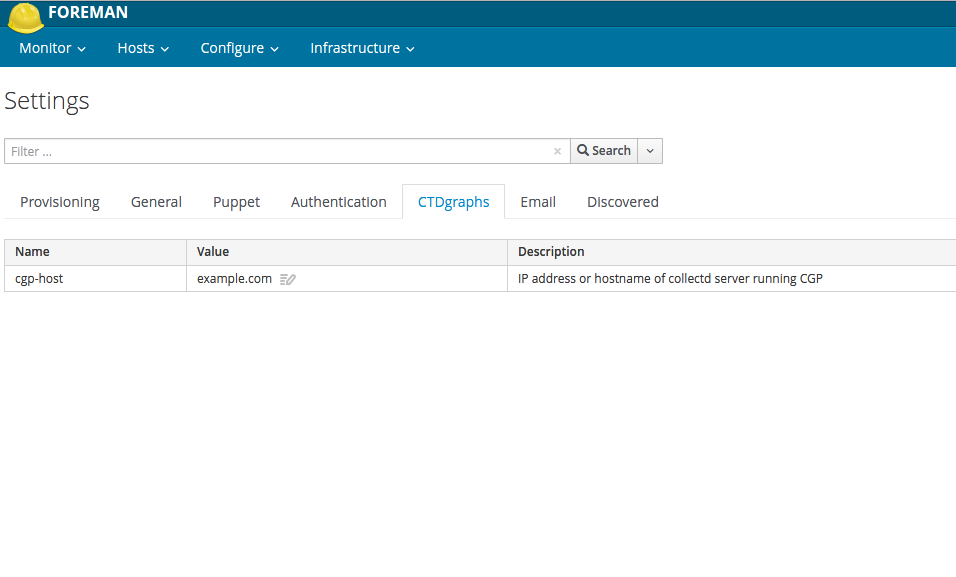
\includegraphics[width=\textwidth]{files/plugin-config.png}
	\caption{Foreman-collectd-graphs-plugin: konfigurace }\label{fig:float}
\end{figure}


\chapter{Manuál pluginu}

\begin{minted}{text}
# Foreman-collectd-plugin

Collectd plugin for foreman showing graphs from collectd graph
panel running on hostname set in config file.

## Installation

See [How_to_Install_a_Plugin](http://projects.theforeman.org/proj
	ects/foreman/wiki/How_to_Install_a_Plugin)
for how to install Foreman plugins

## Config file

create file collectd-graph-plugin.yml in /etc/foreman/plugins
 with following:
```
  :collectd-graph-plugin:
    :hostname: collectd.weedtime.cz/CGP/
```
where on collectd.weedtime.cz/CGP/ is running collectd graph
pannel, see https://github.com/pommi/CGP

## Contributing

Fork and send a Pull Request. Thanks!

## Copyright

Copyright (c) 2017 Jan Sokol GNU GPL 3

\end{minted}


\chapter{Manuál pro ansible}

\begin{minted}{text}
Ansible
-------

 - Installation:
 	http://docs.ansible.com/intro_installation.html
 - Ansible version should be < 2.0

Setup
-----

 1. Clone this repository
 1. Change `hosts` file according to your needs
 1. Change values specified in group_vars/* files

Running playbooks
-----------------

		ansible-playbook -i <hosts_file> <playbook>
		 --check

Example:

		ansible-playbook -i hosts proxy_server.yml
		 --check

Run these without `--check` to apply changes on server.
\end{minted}


\chapter{Seznam použitých zkratek}
% \printglossaries
\begin{description}
	\item[GUI] Graphical user interface
	\item[PXE] Preboot eXecution Environment
	\item[DHCP] Dynamic Host Configuration Protocol
	\item[DNS] Domain Name System
	\item[TFTP] Trivial File Transfer Protocol
	\item[TCP] Transmission Control Protocol
	\item[UDP] User Datagram Protocol
	\item[RHEL] Red Hat Enterprise Linux
	\item[SSL] Secure Sockets Layer
	\item[NIC] Network Interface Controller
	\item[FQDN] Fully Qualified Domain Name
	\item[IPMI] Intelligent Platform Management Interface
	\item[IP] Internet Protocol
	\item[UNDI] Universal Network Device Interface
	\item[UUID] Universally Unique Identifier
	\item[GUID] Globally Unique Identifier
	\item[VLAN] Virtuální LAN
	\item[API] Application Programming Interface
	\item[KVM] Kernel-based Virtual Machine
	\item[XSS] Cross-Site Scripting


	\item[MTFTP] Multicast Trivial File Transfer Protocol
	\item[GRUB] GRand Unified Bootloader
	\item[FAT] File Allocation Table
	\item[HTTP] Hypertext Transfer Protocol
	\item[BIOS] Basic Input-Output System
	\item[MBR] Master Boot Record
	\item[UEFI] Unified Extensible Firmware Interface
	\item[GPT] GUID Partition Table


\end{description}


% % % % % % % % % % % % % % % % % % % % % % % % % % % %
% % Tuto kapitolu z výsledné práce ODSTRAŇTE.
% % % % % % % % % % % % % % % % % % % % % % % % % % % %
%
% \chapter{Návod k~použití této šablony}
%
% Tento dokument slouží jako základ pro napsání závěrečné práce na Fakultě informačních technologií ČVUT v~Praze.
%
% \section{Výběr základu}
%
% Vyberte si šablonu podle druhu práce (bakalářská, diplomová), jazyka (čeština, angličtina) a kódování (ASCII, \mbox{UTF-8}, \mbox{ISO-8859-2} neboli latin2 a nebo \mbox{Windows-1250}).
%
% V~české variantě naleznete šablony v~souborech pojmenovaných ve formátu práce\_kódování.tex. Typ může být:
% \begin{description}
% 	\item[BP] bakalářská práce,
% 	\item[DP] diplomová (magisterská) práce.
% \end{description}
% Kódování, ve kterém chcete psát, může být:
% \begin{description}
% 	\item[UTF-8] kódování Unicode,
% 	\item[ISO-8859-2] latin2,
% 	\item[Windows-1250] znaková sada 1250 Windows.
% \end{description}
% V~případě nejistoty ohledně kódování doporučujeme následující postup:
% \begin{enumerate}
% 	\item Otevřete šablony pro kódování UTF-8 v~editoru prostého textu, který chcete pro psaní práce použít -- pokud můžete texty s~diakritikou normálně přečíst, použijte tuto šablonu.
% 	\item V~opačném případě postupujte dále podle toho, jaký operační systém používáte:
% 	\begin{itemize}
% 		\item v~případě Windows použijte šablonu pro kódování \mbox{Windows-1250},
% 		\item jinak zkuste použít šablonu pro kódování \mbox{ISO-8859-2}.
% 	\end{itemize}
% \end{enumerate}
%
%
% V~anglické variantě jsou šablony pojmenované podle typu práce, možnosti jsou:
% \begin{description}
% 	\item[bachelors] bakalářská práce,
% 	\item[masters] diplomová (magisterská) práce.
% \end{description}
%
% \section{Použití šablony}
%
% Šablona je určena pro zpracování systémem \LaTeXe{}. Text je možné psát v~textovém editoru jako prostý text, lze však také využít specializovaný editor pro \LaTeX{}, např. Kile.
%
% Pro získání tisknutelného výstupu z~takto vytvořeného souboru použijte příkaz \verb|pdflatex|, kterému předáte cestu k~souboru jako parametr. Vhodný editor pro \LaTeX{} toto udělá za Vás. \verb|pdfcslatex| ani \verb|cslatex| \emph{nebudou} s~těmito šablonami fungovat.
%
% Více informací o~použití systému \LaTeX{} najdete např. v~\cite{wikilatex}.
%
% \subsection{Typografie}
%
% Při psaní dodržujte typografické konvence zvoleného jazyka. České \uv{uvozovky} zapisujte použitím příkazu \verb|\uv|, kterému v~parametru předáte text, jenž má být v~uvozovkách. Anglické otevírací uvozovky se v~\LaTeX{}u zadávají jako dva zpětné apostrofy, uzavírací uvozovky jako dva apostrofy. Často chybně uváděný symbol "{} (palce) nemá s~uvozovkami nic společného.
%
% Dále je třeba zabránit zalomení řádky mezi některými slovy, v~češtině např. za jednopísmennými předložkami a spojkami (vyjma \uv{a}). To docílíte vložením pružné nezalomitelné mezery -- znakem \texttt{\textasciitilde}. V~tomto případě to není třeba dělat ručně, lze použít program \verb|vlna|.
%
% Více o~typografii viz \cite{kobltypo}.
%
% \subsection{Obrázky}
%
% Pro umožnění vkládání obrázků je vhodné použít balíček \verb|graphicx|, samotné vložení se provede příkazem \verb|\includegraphics|. Takto je možné vkládat obrázky ve formátu PDF, PNG a JPEG jestliže používáte pdf\LaTeX{} nebo ve formátu EPS jestliže používáte \LaTeX{}. Doporučujeme preferovat vektorové obrázky před rastrovými (vyjma fotografií).
%
% \subsubsection{Získání vhodného formátu}
%
% Pro získání vektorových formátů PDF nebo EPS z~jiných lze použít některý z~vektorových grafických editorů. Pro převod rastrového obrázku na vektorový lze použít rasterizaci, kterou mnohé editory zvládají (např. Inkscape). Pro konverze lze použít též nástroje pro dávkové zpracování běžně dodávané s~\LaTeX{}em, např. \verb|epstopdf|.
%
% \subsubsection{Plovoucí prostředí}
%
% Příkazem \verb|\includegraphics| lze obrázky vkládat přímo, doporučujeme však použít plovoucí prostředí, konkrétně \verb|figure|. Například obrázek \ref{fig:float} byl vložen tímto způsobem. Vůbec přitom nevadí, když je obrázek umístěn jinde, než bylo původně zamýšleno -- je tomu tak hlavně kvůli dodržení typografických konvencí. Namísto vynucování konkrétní pozice obrázku doporučujeme používat odkazování z~textu (dvojice příkazů \verb|\label| a \verb|\ref|).
%
% \begin{figure}\centering
% 	
\includegraphics[width=0.5\textwidth, angle=30]{cvut-logo-bw}
% 	\caption[Příklad obrázku]{Ukázkový obrázek v~plovoucím prostředí}\label{fig:float}
% \end{figure}
%
% \subsubsection{Verze obrázků}
%
% % Gnuplot BW i barevně
% Může se hodit mít více verzí stejného obrázku, např. pro barevný či černobílý tisk a nebo pro prezentaci. S~pomocí některých nástrojů na generování grafiky je to snadné.
%
% Máte-li například graf vytvořený v programu Gnuplot, můžete jeho černobílou variantu (viz obr. \ref{fig:gnuplot-bw}) vytvořit parametrem \verb|monochrome dashed| příkazu \verb|set term|. Barevnou variantu (viz obr. \ref{fig:gnuplot-col}) vhodnou na prezentace lze vytvořit parametrem \verb|colour solid|.
%
% \begin{figure}\centering
% 	\includegraphics{gnuplot-bw}
% 	\caption{Černobílá varianta obrázku generovaného programem Gnuplot}\label{fig:gnuplot-bw}
% \end{figure}
%
% \begin{figure}\centering
% 	\includegraphics{gnuplot-col}
% 	\caption{Barevná varianta obrázku generovaného programem Gnuplot}\label{fig:gnuplot-col}
% \end{figure}
%
%
% \subsection{Tabulky}
%
% Tabulky lze zadávat různě, např. v~prostředí \verb|tabular|, avšak pro jejich vkládání platí to samé, co pro obrázky -- použijte plovoucí prostředí, v~tomto případě \verb|table|. Například tabulka \ref{tab:matematika} byla vložena tímto způsobem.
%
% \begin{table}\centering
% 	\caption[Příklad tabulky]{Zadávání matematiky}\label{tab:matematika}
% 	\begin{tabular}{|l|l|c|c|}\hline
% 		Typ		& Prostředí		& \LaTeX{}ovská zkratka	& \TeX{}ovská zkratka	\tabularnewline \hline \hline
% 		Text		& \verb|math|		& \verb|\(...\)|	& \verb|$...$|		\tabularnewline \hline
% 		Displayed	& \verb|displaymath|	& \verb|\[...\]|	& \verb|$$...$$|	\tabularnewline \hline
% 	\end{tabular}
% \end{table}
%
% % % % % % % % % % % % % % % % % % % % % % % % % % % %

\chapter{Obsah přiloženého CD}

%upravte podle skutecnosti


\begin{figure}
	\dirtree{%
		.1 readme.txt\DTcomment{stručný popis obsahu CD}.
		.1 src.
		.2 plugin\DTcomment{zdrojové kódy pluginu}.
		.2 ansible\DTcomment{konfigurační soubory pro Ansible}.
		.2 thesis\DTcomment{zdrojová forma práce ve formátu \LaTeX{}}.
		.1 text\DTcomment{text práce}.
		.2 thesis.pdf\DTcomment{text práce ve formátu PDF}.
		.2 thesis.ps\DTcomment{text práce ve formátu PS}.
	}
\end{figure}


\end{document}
